\documentclass[hidelinks, a4paper,12pt]{article}
\usepackage{ amsmath, amssymb}
\usepackage{graphicx}
\usepackage{color,amsmath,graphics,graphicx}
\usepackage{amsfonts} % replace subfigure with subcaption instead 
\usepackage{mathrsfs,hyperref}
\usepackage{latexsym,amsmath,enumerate,amsbsy,amsthm,verbatim,enumitem}
\usepackage{amstext,amsopn}
\usepackage{makeidx} 
\textwidth = 415pt

%==============================================
\usepackage{fontspec}
\usepackage{xunicode}
\usepackage{xltxtra}
\defaultfontfeatures{Scale=1.23}
\XeTeXlinebreaklocale “th_TH” % สำหรับตัดคำ
\setmainfont[Scale=1.23]{THSarabunNew}
%==============================================
%%%%%%%%%%%%%%% THEOREM Environments %%%%%%%%%% 
\newtheorem{theorem}{ทฤษฎีบท}[section]						%
\newtheorem{lemma}[theorem]{บทตั้ง}						%
\newtheorem{conjecture}[theorem]{บทคาดการณ์}				%
\newtheorem{definition}[theorem]{บทนิยาม}					%
\newtheorem{remark}[theorem]{หมายเหตุ}						%
\newtheorem{proposition}[theorem]{ประพจน์}					%
\newtheorem{corollary}[theorem]{บทแทรก}					%
\numberwithin{equation}{section}							%
\newtheorem{example}[theorem]{ตัวอย่าง}						%
%\newtheorem{exercise}{แบบฝึกหัด}[chapter]	
%\renewcommand{\chaptername}{บทที่}
\renewcommand\tablename{ตารางที่}
\renewcommand\figurename{รูปที่}
\renewcommand{\contentsname}{สารบัญ}						%
%\renewcommand{\bibname}{บรรณานุกรม}						% 
\renewcommand{\indexname}{ดรรชนี}					%
\counterwithin{figure}{section}
\numberwithin{equation}{section}		
%%%%%%%%%%%%%%%%%%%%%%%%%%%%%%%%%%%%%%%%%%%%%%%
% addition mod
\usepackage{subcaption,float,framed,hyperref}
\usepackage[ruled]{algorithm2e}
% =============

\begin{document}
	{\begin{center}
			\textbf{Report Progress}\\
			\vspace{0.5cm}
			\textbf{Division of Applied Mathematics, Department of Mathematics}\\
			\vspace{0.5cm}
			\textbf{Faculty of Science, Silpakorn University}
		\end{center}}
		{
			\vspace{0.5cm}
			\flushleft{Date : { 23 พฤศจิกายน 2561 } \hfill{ }}
			\flushleft{Advisor : { ผู้ช่วยศาสตราจารย์ ดร.นพดล  ชุมชอบ}}\\
			\flushleft{Student : {นายภัคพล พงษ์ทวี รหัส  07580028}
			\vspace{1cm}
		}
		
		
		% Here the project title
		{\textbf{\begin{flushleft}Project Title : ขั้นตอนวิธีเชิงตัวเลขชนิดใหม่สำหรับการต่อเติมภาพที่ใช้การแปรผันรวมกับการประยุกต์สำหรับซ่อมแซมภาพจิตรกรรมไทยโบราณและการลบบทบรรยายจากอนิเมะ \\
				(A new numerical algorithm for TV-based image inpainting with its applications for restoring ancient Thai painting images and removing subtitles from animes)
			\end{flushleft}
		}}
		\thispagestyle{empty}
	\section{ที่มาและความสำคัญ}
	\hspace{1cm} ในปัจจุบันการใช้ภาพดิจิตัล (digital images) ในสังคมเครือข่ายได้รับความนิยมอย่างแพร่หลาย เนื่องจากโทรศัพท์เคลื่อนที่มีราคาถูกลงแต่มีความสามารถที่ชาญฉลาด สามารถทำหน้าที่ได้ตั้งแต่การเป็นกล้องดิจิตัลคอมแพค (compact digital camera)  คุณภาพดีให้ภาพดิจิตัลที่มีความคมชัดสูงจนไปถึงการทำหน้าที่ดังเช่นเครื่องคอมพิวเตอร์ส่วนบุคคลที่สามารถเชื่อมต่อกับระบบเครือข่ายไร้สายเพื่อรับส่งภาพดิจิตัลในสังคมเครือข่ายด้วยความสะดวกและรวดเร็ว 
	
	\hspace{1cm} นอกจากภาพดิจิตัลจะได้รับจากการถ่ายภาพด้วยโทรศัพท์เคลื่อนที่แล้ว ภาพดิจิตัลยังได้รับการถ่ายภาพด้วยกล้องดีเอสแอลอาร์ หรือ กล้องสะท้อนเลนส์เดี่ยวแบบดิจิตัล (digital single lens reflex camera) กล้องโทรทรรศน์ (หรือ กล้องดูดาว) หรือ เครื่องมือสร้างภาพถ่ายทางการแพทย์ (medical imaging device) 
	
	\hspace{1cm} โดยทั่วไปภาพดิจิตัลจะได้รับการประมวลผลภาพก่อนนำไปใช้งานเพื่อให้สามารถใช้ข้อมูลที่ปรากฎบนภาพได้ตรงวัตถุประสงค์ของการใช้งานมากที่สุด ตัวอย่างเช่น ภาพบุคคล (portrait) อาจจำเป็นต้องได้รับการกำจัดสัญญาณรบกวนออกจากภาพและ/หรือปรับเพิ่มความละเอียดข้อมูลของความเข้มของสีและความสว่างของสีบนบริเวณใบหน้าก่อนนำภาพไปใช้งานเพื่อจัดทำต้นฉบับวารสารหรือหนังสือของสำนักพิมพ์ เป็นต้น  
	
	\hspace{1cm} การต่อเติมภาพ (image inpainting) เป็นวิธีการประมวลผลภาพชนิดหนึ่งมีเป้าหมายเพื่อซ่อมแซมภาพด้วยการต่อเติมข้อมูลของความเข้มของสีบนบริเวณที่กำหนด (ต่อไปจะเรียกบริเวณนี้ว่าโดเมนต่อเติม (inpainting domain)) โดยอาศัยข้อมูลของความเข้มของสีที่ปรากฏในภาพ ตัวอย่างเช่น 
	กำหนดให้รูปที่ \ref{fig1} (a) แสดงภาพที่ต้องการซ่อมแซมระดับความเข้มของสีบนบริเวณแท่งวัตถุรูปร่างสี่เหลี่ยมสีขาว การต่อเติมภาพดังกล่าวจะเริ่มด้วยการกำหนดให้บริเวณแท่งวัตถุรูปร่างสี่เหลี่ยมสีขาวเป็นโดเมนการต่อเติมดังรูปที่ \ref{fig1} (b) จากนั้นภาพที่ได้รับการซ่อมแซมหรือภาพที่ได้รับการต่อเติม (restored or inpainted image) ซึ่งแสดงในรูปที่ \ref{fig1} (c) ได้มาจากขั้นตอนวิธีการต่อเติมภาพ (inpainting algorithm) ซึ่งได้รับการออกแบบเพื่อนำข้อมูลที่ปรากฎบนภาพในบริเวณใกล้เคียงกับขอบของโดเมนต่อเติมมาซ่อมแซมภาพ 
	
	\begin{figure}[H]
		\centering
		\begin{subfigure}{0.3\linewidth}
			\centering
			
\includegraphics[width=0.8\linewidth]{images/grayscale_inpaint/toinpaint.png}
			\caption{ภาพที่ต้องการซ่อมแซม}
		\end{subfigure}
		\begin{subfigure}{0.3\linewidth}
			\centering
			
\includegraphics[width=0.8\linewidth]{images/grayscale_inpaint/inpaintdomain.png}
			\caption{โดเมนต่อเติม}
		\end{subfigure}
		\begin{subfigure}{0.3\linewidth}
			\centering
			
\includegraphics[width=0.8\linewidth]{images/grayscale_inpaint/result_splitbergman.png}
			\caption{ภาพที่ได้รับการซ่อมแซม}
		\end{subfigure}
		\caption{ตัวอย่างการซ่อมแซมภาพ; (a) ภาพที่ต้องการซ่อมแซม; (b) โดเมนต่อเติม; (c) ภาพที่ได้รับการซ่อมแซม}
		\label{fig1}
	\end{figure}
	
	\hspace{1cm} เท่าที่ผู้วิจัยศึกษาและค้นคว้ามาจนถึงขณะนี้ ผู้วิจัยพบว่าการต่อเติมภาพมักนิยมนำไปใช้งานสำหรับการปรับแต่งความสวยงามของภาพบุคคลที่ถ่ายจากโทรศัพท์เคลื่อนที่ เช่น การลบร่องรอยของรอยตีนกา การลบร่องรอยแผลเป็นที่เกิดจากสิวเสี้ยน การลดร่องรอยของความชรา หรือ การเพิ่มความใสและความเนียนของสีผิวบนบริเวณใบหน้าผ่านโปรแกรมแอปพลิเคชันแต่งรูปภาพที่มีอยู่ในแอปสโตร์ (App Store) หรือ กูเกิ้ลเพลย์ (Google Play) เป็นต้น 
	
	\subsection{การซ่อมแซมภาพจิตรกรรมไทยโบราณ}
	
	\hspace{1cm} ภาพจิตรกรรมไทย คือ ภาพเขียนที่มีเอกลักษณ์ความเป็นศิลปะไทยซึ่งโดดเด่นและแตกต่างจากภาพเขียนของชนชาติอื่น ในอดีต  ช่างไทยได้สร้างสรรค์ลวดลายและสีสันบนภาพวาดเพื่อสะท้อนประเพณีและวัฒนธรรมในสังคมไทยที่เกี่ยวกับศาสนา ประวัติศาสตร์ โบราณคดี ชีวิตความเป็นอยู่ วัฒนธรรมการแต่งกาย ตลอดจนการแสดงการเล่นพื้นเมืองต่าง ๆ ของแต่ละยุคสมัย 
	
	\hspace{1cm} อย่างไรก็ตาม ภาพจิตรกรรมไทยจำนวนไม่น้อยที่เสื่อมสลายตามกาลเวลา และรอคอยการซ่อมแซมจากช่างในสมัยปัจจุบันที่ต้องไม่สร้างความเสียหายให้กับภาพเขียนเพิ่มขึ้นมากกว่าเดิม  ที่ผ่านมาภาพที่ผ่านการซ่อมแซมมาแล้วจำนวนไม่น้อยได้รับความเสียหายหลังจากการซ่อมแซม ถึงแม้สภาพโดยรวมของภาพจิตรกรรมเดิมยังคงอยู่ แต่รายละเอียดในตัวภาพเขียนได้เปลี่ยนไป ก่อให้เกิดความเสียหายที่ประเมินค่าไม่ได้ 
	
	\hspace{1cm} การซ่อมแซมภาพจิตรกรรมไทยโบราณโดยใช้การต่อเติมภาพเป็นขั้นตอนของการซ่อมแซมแบบหนึ่งซึ่งไม่ก่อให้เกิดความเสียหายใด ๆ กับภาพเดิม เนื่องจากเป็นการซ่อมแซมโดยการใช้ขั้นตอนวิธีเชิงตัวเลขบนภาพดิจิตัลซึ่งเป็นสำเนาของภาพเดิม ด้วยเหตุผลดังกล่าว ผู้วิจัยได้เล็งเห็นว่าการซ่อมแซมภาพจิตรกรรมไทยโบราณมีความจำเป็นเร่งด่วน เนื่องจากภาพที่ได้รับการซ่อมแซมด้วยการต่อเติมภาพสามารถนำไปใช้ประกอบการตัดสินใจเพื่อวางแผนก่อนการลงมือซ่อมแซมภาพเขียนจริงได้ นอกจากนี้ ขั้นตอนวิธีการต่อเติมภาพสามารถนำไปใช้สร้างแอปพลิเคชันบนโทรศัพท์เคลื่อนที่เพื่อในไปใช้เป็นข้อมูลในการเข้าชมภาพเขียนเดิมที่ยังไม่ได้รับการซ่อมแซมและภาพเขียนที่ได้รับการซ่อมแซมโดยวิธีการทางคณิตศาสตร์จากแอปพลิเคชันที่พัฒนาขึ้น
	
	\hspace{1cm} รูปที่ \ref{fig2} แสดงตัวอย่างภาพจิตรกรรมไทย\footnote{ภาพถ่ายที่วัดภูมินทร์ อำเภอเมือง จังหวัดน่าน; ภาพจาก http://topicstock.pantip.com/camera/topicstock/2009/02/O7514399/O7514399.html สืบค้นเมื่อวันที่ 23 กันยายน 2561} ที่ต้องได้รับการซ่อมแซมบนบริเวณแขนเสื้อของรูปวาดผู้ชายที่มีส่วนของสีแดงเดิมหลุดหายไป ทั้งนี้ในการซ่อมแซมภาพโดยการต่อเติมภาพ เราจะเริ่มด้วยการสร้างโดเมนต่อเติมบนบริเวณสีพื้นผิวปูนที่แขนเสื้อ จากนั้นจึงนำขั้นตอนวิธีการต่อเติมภาพเพื่อซ่อมแซมภาพบริเวณนั้นให้เป็นสีแดง 
	
	\begin{figure}[h]
		\[
		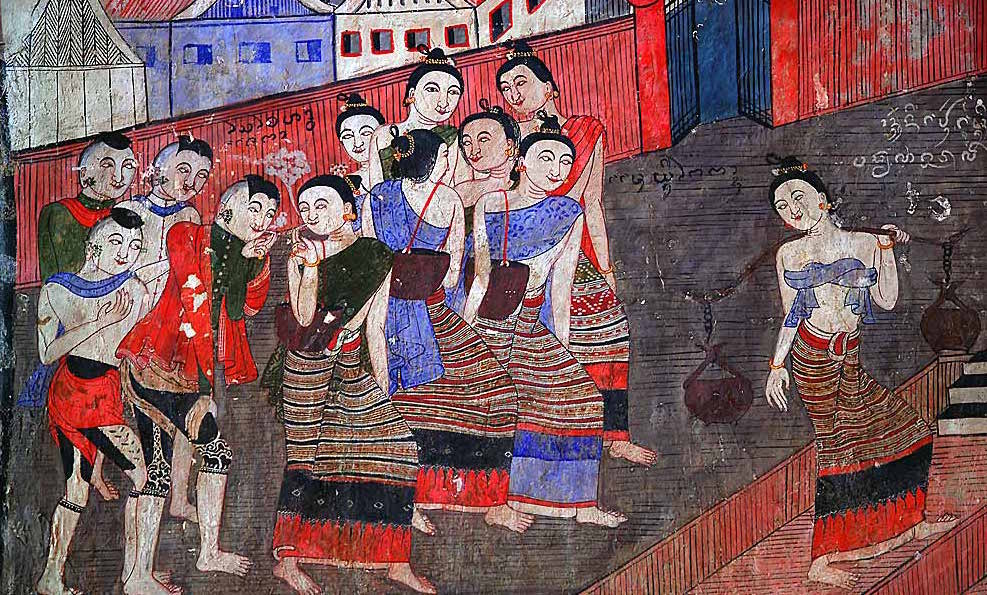
\includegraphics[width=0.6\linewidth]{images/show_peicewise/fig2a.jpg}
		\]
		\caption{ภาพจิตรกรรมไทยที่วัดภูมินทร์ อำเภอเมือง จังหวัดน่าน}
		\label{fig2}
	\end{figure}
	
	
	\subsection{การลบบทบรรยายบนอนิเมะ}
	\hspace{1cm}อนิเมะคือวิดีโอภาพวาดการ์ตูนสไตล์ญี่ปุ่นซึ่งเป็นที่นิยมของเยาวชนไทย ในการรับชมอนิเมะ แม้ว่าเยาวชนไทยสามารถรับชมด้วยบทพากย์เสียงภาษาไทย แต่ก็สูญเสียอรรถรสของการรับชมจากบทบรรยายแบบแข็ง\footnote{บทยรรยายที่ไม่สามารถปิดหรือเปิดได้} (hardsub) ที่เป็นภาษาต่างประเทศในบริเวณด้านล่างของจอภาพ ในการซ่อมแซม\\อนิเมะด้วยการลบบทบรรยายภาษาต่างประเทศจึงเป็นงานที่ยุ่งยากและท้าท้ายมาก เนื่องจาก
	\begin{itemize}
		\item [(1)] อนิเมะเป็นวิดีโอซึ่งแสดงผลประมาณ 24 เฟรม(ภาพ)ต่อวินาที
		\item [(2)] แต่ละเฟรมอาจมีหรืออาจไม่มีบทบรรยายก็ได้
		\item [(3)] แต่ละเฟรมอาจมีหรืออาจไม่มีบทบรรยายเดียวกันก็ได้
		\item [(4)] แต่ละเฟรมเป็นการแสดงผลภาพสีที่มีระดับความคมชัดสูง (high definition) ขนาดมากถึง $1920\times1080$ พิกเซล
	\end{itemize}
	ด้วยความท้าทายข้างต้น การพัฒนาขั้นตอนวิธีการต่อเติมภาพที่สามารถกำหนดโดเมนต่อเติมเชิงอัตโนมัติให้กับแต่ละเฟรมและประมวลผลได้แม่นยำจนการลบบทบรรยายสามารถทำงานได้แบบเรียลไทม์จึงเป็นสิ่งจำเป็นที่หลีกเลี่ยงไม่ได้
	
	\hspace{1cm} รูปที่ \ref{fig3} แสดงตัวอย่าง 1 เฟรมของอนิเมะที่มีบทบรรยายแบบแข็ง\footnote{ภาพจาก https://www.samehadaku.tv/2018/07/grand-blue-episode-1-subtitle-indonesia.html สืบค้นเมื่อวันที่ 23 กันยายน 2561} ที่ต้องซ่อมแซมด้วยการลบบทบรรยายออก  ทั้งนี้ในการลบบทบรรยายออกจากเฟรมโดยใช้การต่อเติมภาพ เราจะเริ่มด้วยการสร้างโดเมนต่อเติมแบบอัตโนมัติในบริเวณบทบรรยาย จากนั้นจึงนำขั้นตอนวิธีการต่อเติมภาพแบบเร็วเพื่อลบบทบรรยายออกจากเฟรม 
	
	\begin{figure}[h]
		\[
		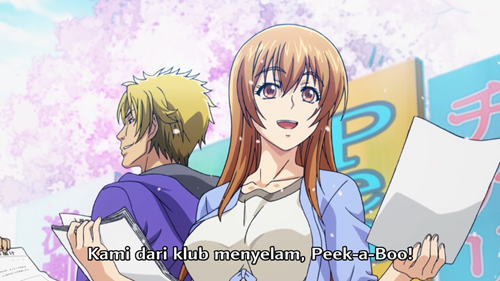
\includegraphics[width=0.6\linewidth]{images/show_peicewise/fig3.png}
		\]
		\caption{1 เฟรมของอนิเมะที่มีบทบรรยายแบบแข็ง}
		\label{fig3}
	\end{figure}
	
	\hspace{1cm} โครงการวิจัยนี้ ผู้วิจัยมีเป้าหมายสำคัญคือการพัฒนาขั้นตอนวิธีการต่อเติมภาพแบบเร็วและแม่นยำชนิดใหม่เพื่อนำไปใช้สำหรับซ่อมแซมภาพจิตรกรรมไทยและการลบบทบรรยายออกจากอนิเมะ


\section{วรรณกรรมและทฤษฎีบทที่เกี่ยวข้อง} 
\hspace{1cm} ในการกล่าวถึงขั้นตอนวิธีการต่อเติมภาพ จะเริ่มต้นด้วยการกล่าวทบทวนเกี่ยวกับการต่อเติมภาพเฉดสีเทา (grayscale image) ก่อน ดังนี้

\hspace{1cm} ให้ $\Omega \subset \mathbb{R}^2$ แทนโดเมนภาพ (image domain) $D \subset \mathbb{R}^2$ แทนโดเมนต่อเติม (ดูรูปที่ \ref{fig4}) และ $V \subset [0,\infty)$ 

\hspace{1cm} ให้ $ u: \Omega \rightarrow V,\ z: \Omega \rightarrow V$ แทนภาพที่ได้รับการซ่อมแซมและภาพที่ต้องการซ่อมแซม ตามลำดับ

\hspace{1cm} ในที่นี้ $ \mathbf{x} = (x,y) \in \Omega $ แทนพิกัดทางกายภาพ (physical position) ของภาพ และ $ u(\mathbf{x}) \in V $ แทนระดับความเข้มของภาพ (image intensity) ที่ $ \mathbf{x} $ และ $ \Omega $ มีรูปร่างสี่เหลี่ยม 

\hspace{1cm} นอกจากนี้เราสามารถสมมติได้โดยไม่เสียหลักการสำคัญว่า $ \Omega = [1,n]^2 $ และ $ V = [0,1] $ เมื่อ $n>0$ เป็นจำนวนเต็มบวก ทั้งนี้ เราจะเรียกภาพ $u,z$ ที่นิยามข้างต้นว่าภาพเฉดสีเทา
\begin{figure}[H]
	\centering
	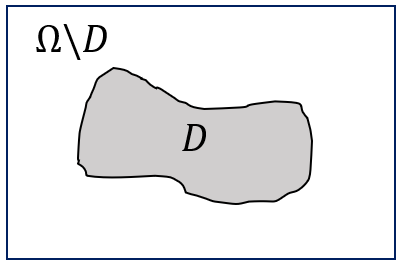
\includegraphics[width=0.4\linewidth]{images/sample-domain.png}
	\caption{$D$ แทนโดเมนต่อเติม}
	\label{fig4}
\end{figure}

\subsection{ตัวแบบการต่อเติมภาพเฉดสีเทาที่ใช้การแปรผันรวม}\label{inpaint-model-grayscale}

\hspace{1cm} ในการต่อเติมภาพเฉดสีเทา Chan และ Shen \cite{ref:rof-inpaint-chan-shen} ได้นำเสนอตัวแบบเชิงการแปรผัน (variational model) ที่ใช้เร็กกิวลาร์ไรซ์เซชันแบบการแปรผันรวม (Total variation based regularization) โดยพัฒนาต่อจากตัวแบบ ROF สำหรับการกำจัดสัญญาณรบกวน \cite{ref:ROF-template} ซึ่งตัวแบบเชิงการแปรผันนี้กำหนดโดย
\begin{align}
\min_{u} \{ \mathcal{J}(u) = \frac{1}{2} \int_{\Omega}\lambda (u-z)^2 d\Omega +  \int_{\Omega}  |\nabla u|  d\Omega \}
\label{e1}
\end{align}
เมื่อ 
\begin{align}
\lambda=\lambda(\mathbf{x}) = \left \{ \begin{array}{ll}  \lambda_0, & x \in \Omega \textbackslash D \\ 0, & x \in D  \end{array} \right . 
\label{e2}
\end{align}
แทนพารามิเตอร์เร็กกิวลาร์ไรซ์เซชัน (regularization parameter) และ $\lambda_0 >0$

\hspace{1cm} โดยแคลคูลัสของการแปรผัน (Calculus of variations) จะได้สมการออยเลอร์ลากรางจ์ที่เกี่ยวข้องกับ (\ref{e1}) เป็น 
\begin{align}
\left \{ \begin{array}{ll}  - \nabla \cdot  \Big( \dfrac{\nabla u}{|\nabla u|} \Big) + \lambda (u-z) = 0,  & \hspace{1cm} \mathbf{x} \in (1,n)^2 \\ \dfrac{\partial u}{\partial \boldsymbol{n}} = 0, & \hspace{1cm} x \in \partial \Omega \end{array} \right . 
\label{e3}
\end{align}
เมื่อ $\boldsymbol{n}$ แทนเวกเตอร์หน่วยที่ตั้งฉากกับของของภาพ

\hspace{1cm} ต่อไปจะกล่าวทบทวนวิธีการเชิงตัวเลขสำหรับแก้สมการเชิงอนุพันธ์ย่อยใน (\ref{e3}) 
\begin{itemize}
	\item[(1)] วิธีการเดินเวลาแบบชัดแจ้ง (explicit time marching method) 
	
	\hspace{1cm} คณะวิจัย \cite{ref:ROF-template} ได้แนะนำวิธีการเชิงตัวเลขสำหรับการกำจัดสัญญาณรบกวนโดยใช้วิธีการเดินเวลาแบบชัดแจ้ง ซึ่งสามารถประยุกต์เป็นวิธีเชิงตัวเลขสำหรับการต่อเติมภาพได้ดังนี้
	
	\hspace{1cm} เริ่มจากการแนะนําตัวแปรเวลาสังเคราะห์ (time artificial variable) จากนั้นหาคําตอบแบบสภาวะคงตัว (steady-state solution) ในขณะที่ $t\rightarrow \infty$ ของสมการเชิงอนุพันธ์ย่อยไม่เป็นเชิงเส้นที่ขึ้นอยู่กับเวลา 
	\begin{align}
	u(\mathbf{x},t_{k+1})=u(\mathbf{x},t_{k})+\tau\left(\nabla \cdot\left(\dfrac{\nabla u (\mathbf{x},t_k)}{| \nabla u (\mathbf{x},t_k) | }\right) + \lambda(\mathbf{x})(u (\mathbf{x},t_k)-z(\mathbf{x})) \right),\ u(\mathbf{x},t_0)=z
	\label{e4}
	\end{align}
	เมื่อ $t_k=t_0+k\tau\ (\tau>0)$  แทนขั้นเวลาที่ $k$ และ $t_0=0$ แทนขั้นเวลาเริ่มต้น
	
	 \vspace{0.5cm} \hspace{0.5cm}วิธีเดินเวลาแบบชัดแจ้งสำหรับภาพเฉดเทามีขั้นตอนวิธีดังนี้  \\
	 \vspace{0.5cm} 
	\begin{algorithm}[H]
		\caption{ETM Method for TV-based Image Inpainting}		
		\SetKwFunction{FMain}{$u \longleftarrow ETM$}\SetAlgoNoLine 
		\SetKwProg{Fn}{}{}{}
		\Fn{\FMain{$u,z,\lambda,\beta,\tau,N,\varepsilon$}}{
			\textbf{initialize}
			$i = 0$; $z = u$; $err = 1$\\
			\While{$ i < N $ \textbf{and} $err > \varepsilon$}{
				$u^{old} = u$\\
				$u = u + \tau\left(\nabla \cdot\left(\dfrac{\nabla u}{\sqrt{u_x^2 + u_y^2+ \beta}}\right) + \lambda(u-z) \right)$ \\ 		
				$err = \frac{||u-u^{old}||}{||u||}$ \\
				$ i = i + 1 $
			}
		}
	\end{algorithm}
	
	 \item[(2)] วิธีการทำซ้ำแบบจุดตรึง (fixed-point iteration method) 
	 
	 \hspace{1cm} คณะวิจัย \cite{ref:FixpointSolver} ได้แนะนำวิธีการเชิงตัวเลขสำหรับการกำจัดสัญญาณรบกวนโดยใช้วิธีการทำซ้ำแบบจุดตรึง ซึ่งสามารถประยุกต์เป็นวิธีเชิงตัวเลขสำหรับการต่อเติมภาพได้ดังนี้
	
	\hspace{1cm} เริ่มจากแนะนำดัชนีการทำซ้ำแบบจุดตรึง $\nu=0,1,2,\cdots$ และนิยามรูปแบบการทำซ้ำโดย
	\begin{align}
	- \nabla\cdot\left(\dfrac{\nabla u^{[\nu+1]}}{{| \nabla u |}^{[v]} }\right) + \lambda(u^{[\nu+1]}-z)  = 0,\ u^{[0]}=z
	\label{e5}
	\end{align}

\hspace{1cm} เนื่องจาก $\tfrac{1}{| \nabla u |}=\tfrac{1}{\sqrt{u_x^2+u_y^2}} \rightarrow \infty$ ในบริเวณที่ $u$ มีความเข้มสีเป็นเอกพันธ์ุ ($u(\mathbf{x})=$ ค่าคงตัว) เพื่อหลีกเลี่ยงปัญหาเชิงตัวเลขจะเกิดขึ้นใน (\ref{e4}) และ (\ref{e5}) เราจะใช้ 
\begin{align*}
|\nabla u| \approx| \nabla u |_\beta=\sqrt{u_x^2+u_y^2+\beta},\ 0< \beta \ll 1
 \end{align*}

\clearpage
\hspace{1cm}วิธีการทำซ้ำแบบจุดตรึงมีขั้นตอนดังนี้ \\
\vspace{0.5cm} 
\begin{algorithm}[H]
	\SetAlgoNoLine
	\caption{FP Method for TV-based Image Inpainting}	
	\SetKwFunction{FMain}{$u \longleftarrow FP$}
	\SetKwProg{Fn}{}{}{}
	\Fn{\FMain{$u, z,\lambda, \beta, N, \varepsilon$}}{		
		\textbf{initialize} $i=0$;$u = z$;$err = 1 $\\
		\While{$ i < N $ \textbf{and} $err > \varepsilon$}{
			$ u^{old} = u$ \\
			$u = GS(u, z, \lambda, \beta, N_{gs})$\\
			$err = \frac{||u-u^{old}||}{||u||}$ \\
			$ i = i + 1 $
		}
	}
	\SetKwFunction{FMain}{$u \longleftarrow GS$}
	\Fn{\FMain{$u, z, \lambda, \beta, N_{gs}$}}{
		\textbf{initialize} $k = 0$\\
		compute $D(u)_{i,j} = \frac{1}{\sqrt{u_x^2+u_y^2+\beta}}, 1 \leq i \leq n_x, 1 \leq j \leq n_y$\\
		\While{$k < N_{gs}$}{
				$u_{i,j}^{k+1} = \frac{\lambda_{i,j}z_{i,j}+                (D_{i,j}(u_{i+1,j}^k+u_{i,j+1}^k)+D_{i-1,j}u_{i-1,j}^{k+1}+D_{i,j-1}u_{i,j-1}^{k+1})}{
				\lambda_{i,j}+(2D_{i,j}+D_{i-1,j}+D_{i,j-1})}$\\
				$k = k+1$
		}
	}
\end{algorithm}
\vspace{0.5cm}
\hspace{1cm} จาก (\ref{e4}) และ (\ref{e5}) เราพบว่ายิ่ง $\beta$ มีค่าน้อยลงมากขึ้นเท่าไหร่ ความแม่นยำของตัวแบบ (\ref{e1}) ยิ่งมีมากขึ้นเท่านั้น นอกจากนี้ เรายังพบอีกว่า การแก้สมการ (\ref{e4}) และ (\ref{e5}) ยิ่งมีความยุ่งยากมากขึ้นสำหรับ $\beta$ ที่มีค่าน้อยๆ 

\hspace{1cm} เพื่อเอาชนะความยากเชิงตัวเลขนี้ คณะวิจัยโดย \cite{ref:splitbergman-inpaint} ได้แนะนำวิธีการสปริทเบรกแมนซึ่งสามารถกล่าวถึงพอสังเขป ดังนี้ \\

\item[(3)] วิธีการสปริทเบรกแมน (Split Bregman method) 

\hspace{1cm} เริ่มจากการแนะนำเวกเตอร์เสริม $\boldsymbol{w}$ พารามิเตอร์เบรกแมน (Bregman parameter) $\boldsymbol{b}$ และพารามิเตอร์เพนัลที (panalty parameter) $\theta>0$ และเขียน (\ref{e1}) ใหม่ ดังนี้
	\begin{align}
	\min_{u,\boldsymbol{w}} \{ \mathcal{J}(u,\boldsymbol{w}) = \dfrac{1}{2} \int_{\Omega} \lambda(u-z)^2 d\Omega +  \int_{\Omega}  | \boldsymbol{w}|  d\Omega + \frac{\theta}{2} \int_{\Omega} (\boldsymbol{w} - \nabla u + \boldsymbol{b}) d\Omega \}
	\label{e6}
	\end{align}
	\hspace{1cm}สำหรับการหาคำตอบของ (\ref{e6}) เราจะใช้วิธีการหาค่าต่ำที่สุดแบบสลับ (alternating minimization method) โดยเริ่มจากการตรึง $\boldsymbol{w}^{\text{old}}$ และ $\boldsymbol{b}^{\text{old}}$ จากนั้นแก้ปัญหาย่อยสำหรับ $u$
	\begin{align}
	u^{\text{New}}=\underset{u}{\arg\min} \{ \mathcal{J}_1(u) = \dfrac{1}{2} \int_{\Omega} \lambda(u-z)^2 d\Omega + \frac{\theta}{2} \int_{\Omega} (\boldsymbol{w}^{\text{old}} - \nabla u + \boldsymbol{b}^{\text{old}}) d\Omega \}
	\label{e7}
	\end{align}
	ต่อไปใช้ $u^{\text{New}}$ ที่ได้จากการแก้ปัญหาย่อย (\ref{e7}) เพื่อแก้ปัญหาย่อยสำหรับ $\boldsymbol{w}$
	\begin{align}
	\boldsymbol{w}^{\text{New}}=\underset{\boldsymbol{w}}{\arg\min} \{ \mathcal{J}_2(\boldsymbol{w}) = \int_{\Omega}  |\boldsymbol{w}|  d\Omega  + \frac{\theta}{2} \int_{\Omega} (\boldsymbol{w} - \nabla u^{\text{New}} + \boldsymbol{b}^{\text{old}}) d\Omega \}
	\label{e8}
	\end{align}
	สุดท้ายจึงปรับปรุงพารามิเตอร์เบรกแมนโดย 
	\begin{align}
	\boldsymbol{b}^{\text{New}}=\boldsymbol{b}^{\text{old}}+\nabla u^{\text{New}}-\boldsymbol{w}^{\text{New}}
	\label{e9}
	\end{align}
	ดำเนินการเช่นนี้จนกระทั่ง $||u^{\text{new}}-u^{\text{old}}||< \epsilon_1$ หรือ $\text{New}>\epsilon_2$ เมื่อ $\epsilon_1,\epsilon_2>0$ \\ 
	\vspace{0.5cm}
	\hspace{1cm}วิธีการสปริทเบรกแมนมีขั้นตอนวิธีดังนี้ \\
	\vspace{0.5cm}
	\begin{algorithm}[H]
		\SetAlgoNoLine
		\caption{SB method for TV-based Image Inpainting}    
		\SetKwFunction{FMain}{$u \longleftarrow SB$}
		\SetKwProg{Fn}{}{}{}
		
		\Fn{\FMain{$u, u_{0}, z,\lambda, \theta, N_{gs}, N, \varepsilon$}}{
			\textbf{initialize}
			$i = 0$,
			$\boldsymbol{b} = \vec{0}$,
			$\boldsymbol{w} = \vec{0}$,
			$u = u_{0}$ \\
			\While{$ i < N $ \textbf{and} $err > \varepsilon$}{
				$u^{old} = u$; 
				$w^{old} = w$;
				$b^{old} = b$;
				 \\
				$u=\underset{u}{\arg\min} \{ \mathcal{J}_1(u) = \dfrac{1}{2} \int_{\Omega} \lambda(u-z)^2 d\Omega + \frac{\theta}{2} \int_{\Omega} (\boldsymbol{w}^{\text{old}} - \nabla u + \boldsymbol{b}^{\text{old}}) d\Omega \}$ \\
				$w =\underset{\boldsymbol{w}}{\arg\min} \{ \mathcal{J}_2(\boldsymbol{w}) = \int_{\Omega}  | \boldsymbol{w}|  d\Omega  + \frac{\theta}{2} \int_{\Omega} (\boldsymbol{w} - \nabla u^{\text{New}} + \boldsymbol{b}^{\text{old}}) d\Omega \}$\\
				$ b = b^{old} + \nabla u - \boldsymbol{w} $ \\
				$err = \frac{||u-u^{old}||}{||u||}$ \\
				$ i = i + 1 $ \\
			}
		}
	\end{algorithm}
	\vspace{0.5cm}
	\textbf{หมายเหตุ:}
	\begin{itemize}
		\item [(1)] ผลเฉลยของ $ u = \underset{u}{\arg\min} \mathcal{J}_1(u) $ กำหนดโดยการแก้ปัญหาผลเฉลยของ
		 $$ - \theta \triangle u + \lambda u = \lambda z - \theta \nabla \cdot (\boldsymbol{w}-\boldsymbol{b})$$ 
		 โดยใช้วิธีการไฟไนต์ดิฟเฟอเรนจ์และวิธีการเกาส์-ไซเดลจำนวน $N_{gs}$ รอบ
		\item [(2)] ผลเฉลยของ $ \boldsymbol{w} = \underset{\boldsymbol{w}}{\arg\min} \mathcal{J}_2(\boldsymbol{w}) $ กำหนดโดย $$\boldsymbol{w} = max\bigg\{(\nabla u + \boldsymbol{b}) - \frac{1}{\theta},0\bigg\}$$
	\end{itemize}
\end{itemize}
\clearpage
\subsection{ตัวแบบการต่อเติมภาพสีที่ใช้การแปรผันรวม}\label{inpaint-model-color}

\hspace{1cm} ต่อไปเราจะพิจารณาภาพสีในระบบสี RGB นั่นคือ เราสมมติว่า

$$ \boldsymbol{u} = (u_1,u_2,u_3)^{\top},\ \boldsymbol{z} = (z_1,z_2,z_3)^{\top} : \Omega  \rightarrow V^3 $$

\noindent เมื่อ $u_1,u_2,u_3: \Omega  \rightarrow V$ และ $z_1,z_2,z_3: \Omega  \rightarrow V$ แทนภาพในเฉดสีแดง สีเขียว และสีน้ำเงินของ $\boldsymbol{u},\boldsymbol{z}$ ตามลำดับ 

\hspace{1cm} ในทำนองเดียวกันกับตัวแบบการต่อเติมภาพเฉดสีเทาที่ใช้การแปรผันรวม ตัวแบบการต่อเติมภาพสีที่ใช้การแปรผันรวมสามารถเขียนได้ดังนี้
\begin{align}
\min_{\boldsymbol{u}} \{ \bar{\mathcal{J}}(\boldsymbol{u})= \mathcal{\bar{D}}(\boldsymbol{u},\boldsymbol{z})+  \mathcal{\bar{R}}(\boldsymbol{u}) \}
\label{e10}
\end{align}
เมื่อ
\begin{align*}
\mathcal{\bar{D}}(\boldsymbol{u},\boldsymbol{z}) 
&= \frac{1}{2}\int_{\Omega}^{}\lambda(u_1 - z_1)^2 d\Omega + \frac{1}{2}\int_{\Omega}^{}\lambda(u_2 - z_2)^2 d\Omega + \frac{1}{2}\int_{\Omega}^{}\lambda(u_3 - z_3)^2 d\Omega
\end{align*}
และ 
\begin{align*}
\mathcal{\bar{R}}(\boldsymbol{u})= \int_{\Omega}^{}\lvert\nabla u_1 \rvert d\Omega + \int_{\Omega}^{}\lvert\nabla u_2 \rvert d\Omega + \int_{\Omega}^{}\lvert\nabla u_3 \rvert d\Omega
\end{align*}

\hspace{1cm}  หลังจากใช้วิธีสปิทเบรกแมนกับ (\ref{e10}) จะได้
\begin{align}
\min_{\boldsymbol{u},\boldsymbol{w}_1,\boldsymbol{w}_2,\boldsymbol{w}_3} \{\bar{\mathcal{J}}(\boldsymbol{u},\boldsymbol{w}_1,\boldsymbol{w}_2,\boldsymbol{w}_3)&= \mathcal{\bar{D}}(\boldsymbol{u},\boldsymbol{z}) +  \underset{l=1}{\overset{3}{\sum}} \int_{\Omega}^{}|\boldsymbol{w}_l|d\Omega
\nonumber\\
&\quad+ \frac{\theta_l}{2} \underset{l=1}{\overset{3}{\sum}}\int_{\Omega}^{}(\boldsymbol{w}_l - \nabla u_l - \boldsymbol{b_l})^{2}d\Omega\}, \hspace{1cm} \theta_l > 0
\end{align}

\vspace{1cm}
\hspace{1cm}ขั้นตอนวิธีสปริทเบรกแมนสำหรับภาพสี แสดงได้ดังนี้ 
\vspace{0.5cm}

\begin{algorithm}[H]
	\SetAlgoNoLine
	\caption{SB Method for Color TV-based Image Inpainting}
	\SetKwFunction{FMain}{$\boldsymbol{u} \longleftarrow SBC$}
	\SetKwProg{Fn}{}{}{}
	\Fn{\FMain{$\boldsymbol{u}, \boldsymbol{z} \lambda, \theta, N_{gs}, N, \varepsilon$}}{
		\For{$l = 1:3$}{
		$u_l \longleftarrow SB(u_l, z_l \lambda, \theta, N_{gs}, N, \varepsilon) $
		}
	}
\end{algorithm}
\vspace{1cm}
\subsection{การวัดประสิทธิภาพของภาพที่ผ่านกระบวนการต่อเติม}

\hspace{1cm} การประเมินคุณภาพของการต่อเติมภาพของวิธีการเชิงตัวเลข จะใช้ค่า PSNR \cite{ref:PSNR} และ SSIM \cite{ref:SSIM} โดย

\begin{align*}
	 \text{PSNR}  &= 10 \cdot log_{10} ( \frac{1}{\sqrt{\text{MSE}}} ) \\
	\text{SSIM}(u,\tilde{u}) &= \frac{(2\mu_u\mu_{\tilde{u}} + 0.0001)(2\sigma_{u\tilde{u}} + 0.0009)}{(\mu_u^2+\mu_{\tilde{u}}^2+0.0001)(\sigma_u^2+\sigma_{\tilde{u}}^2+0.0009)}
\end{align*}

\begin{itemize}
	\item[$\bullet$] MSE คือค่าคลาดเคลื่อนกำลังสองเฉลี่ยของภาพ โดยที่ MSE = $\bigg( \frac{1}{nx \times ny} \sum (u - \bar{u})^2  \bigg)$
	\item[$\bullet$] $u$ แทนภาพต้นฉบับ
	\item[$\bullet$] $\tilde{u}$  แทนภาพต้นฉบับ และภาพที่ได้จากการซ่อมแซมโดยวิธีเชิงตัวเลข
	\item[$\bullet$] $\mu_u$ คือค่าเฉลี่ยของ $u$
	\item[$\bullet$] $\mu_{\tilde{u}}$ คือค่าเฉลี่ยของ $\tilde{u}$
	\item[$\bullet$]  $\sigma_u$ คือความแปรปรวนของ $u$ 
	\item[$\bullet$] $\sigma_{\tilde{u}}$ คือความแปรปรวนของ $\tilde{u}$
\end{itemize}

\textbf{หมายเหตุ:}
\begin{itemize}
	\item [(1)] ถ้า $\tilde{u} \longrightarrow u $ แล้ว PSNR $\longrightarrow \infty$ หมายถึง ภาพที่ซ่อมแซม $\tilde{u}$ มีคุณภาพดี
	\item [(2)] ถ้า $SSIM(u,\tilde{u}) = 1 $
	หมายถึง ภาพที่ซ่อมแซม $\tilde{u}$ มีคุณภาพดี
\end{itemize}


\vspace{1cm}

\section{ผลการดำเนินงานเบื้องต้น}
	\subsection{การซ่อมแซมภาพจิตรกรรมไทยโบราณ}
	\hspace{1cm} สำหรับการซ่อมแซมจิตรกรรมไทยโบราณ ผู้วิจัยจะเริ่มจากการทำการปรับปรุงขั้นตอนวิธีเชิงตัวเลขที่มีอยู่แล้ว โดยใช้ภาพสีที่ได้สังเคราะห์ขึ้นทั้งสิ้น 5 ภาพ โดยแต่ละภาพมีขนาด 256 x 256 พิกเซล ดังรูปที่ \ref{image:synart_original}
	\begin{figure}[H]
		\centering
		\begin{subfigure}{0.4\linewidth}
			\centering
			
\includegraphics[width=0.8\linewidth]{images/image_inpaint_synthetic/case01-original.png}
		\end{subfigure}
		\begin{subfigure}{0.4\linewidth}
			\centering
			
\includegraphics[width=0.8\linewidth]{images/image_inpaint_synthetic/case02-original.png}
		\end{subfigure}
		\bigskip
		\begin{subfigure}{0.4\linewidth}
			\centering
			
\includegraphics[width=0.8\linewidth]{images/image_inpaint_synthetic/case03-original.png}			
		\end{subfigure}
		\begin{subfigure}{0.4\linewidth}
			\centering
			
\includegraphics[width=0.8\linewidth]{images/image_inpaint_synthetic/case04-original.png}			
		\end{subfigure}
		\bigskip
		\begin{subfigure}{0.4\linewidth}
			\centering
			
\includegraphics[width=0.8\linewidth]{images/image_inpaint_synthetic/case05-original.png}			
		\end{subfigure}
		\caption{ภาพต้นฉบับ}
		\label{image:synart_original}
	\end{figure}
	\begin{figure}[H]
		\centering
		\begin{subfigure}{0.4\linewidth}
			\centering
			
\includegraphics[width=0.8\linewidth]{images/image_inpaint_synthetic/case01-toinpaint.png}
		\end{subfigure}
		\begin{subfigure}{0.4\linewidth}
			\centering
			
\includegraphics[width=0.8\linewidth]{images/image_inpaint_synthetic/case02-toinpaint.png}
		\end{subfigure}
		\begin{subfigure}{0.4\linewidth}
			\centering
			
\includegraphics[width=0.8\linewidth]{images/image_inpaint_synthetic/case03-toinpaint.png}		
		\end{subfigure}
		\bigskip
		\begin{subfigure}{0.4\linewidth}
			\centering
			
\includegraphics[width=0.8\linewidth]{images/image_inpaint_synthetic/case04-toinpaint.png}		
		\end{subfigure}
		\begin{subfigure}{0.4\linewidth}
			\centering
			
\includegraphics[width=0.8\linewidth]{images/image_inpaint_synthetic/case05-toinpaint.png}		
		\end{subfigure}
		\caption{ภาพที่จะทำการซ่อมแซม}
	\end{figure}
	\subsubsection{การเปรียบเทียบประสิทธิภาพขั้นตอนวิธีเชิงตัวเลขที่มีอยู่แล้ว}
	
	\hspace{1cm}
	การทดสอบประสิทธิภาพจะใช้ $\varepsilon = 1 \times 10^{-4}$ และ $N= 10,000$ โดยรูปที่ \ref{result:image-timemarching} - \ref{result:image-splitbregman} และตารางที่ \ref{result:table-timemarching} - \ref{result:table-splitbregman} แสดงผลการซ่อมแซมภาพสังเคราะห์ทั้ง 5 ภาพ
	\begin{figure}[H]
		\centering
		\begin{subfigure}{0.4\linewidth}
			\centering
			
\includegraphics[width=0.8\linewidth]{images/result_ex1/timemarch01.png}
		\end{subfigure}
		\begin{subfigure}{0.4\linewidth}
			\centering
			
\includegraphics[width=0.8\linewidth]{images/result_ex1/timemarch02.png}
		\end{subfigure}
		\begin{subfigure}{0.4\linewidth}
			\centering
			
\includegraphics[width=0.8\linewidth]{images/result_ex1/timemarch03.png}			
		\end{subfigure}
		\begin{subfigure}{0.4\linewidth}
			\centering
			
\includegraphics[width=0.8\linewidth]{images/result_ex1/timemarch04.png}			
		\end{subfigure}
		\begin{subfigure}{0.4\linewidth}
			\centering
			
\includegraphics[width=0.8\linewidth]{images/result_ex1/timemarch05.png}			
		\end{subfigure}
		\caption{ผลการซ่อมแซมจากวิธีการเดินเวลา}
		\label{result:image-timemarching}
	\end{figure}
\begin{table}[H]
	\centering
	\begin{tabular}[ht]{|c|c|c|c|c|}
		\hline
		รูปภาพ &เวลาประมวล  (วินาที) & PSNR (dB) & SSIM \\
		\hline
		1 & 82.40 & 25.17 & 0.9997 \\ 
		2 & 127.36 & 17.92 & 0.9980 \\
		3 &  116.39 & 13.33 & 0.9941 \\
		4 & 160.59  &12.40  & 0.9927 \\
		5 & 116.66  & 14.79  & 0.9958 \\
		\hline
		เฉลี่ย & 120.68  & 16.72  & 0.9960 \\
		\hline
	\end{tabular}
	\caption{ผลการซ่อมแซมวิธีการเดินเวลา}
	\label{result:table-timemarching}
\end{table}	
\begin{figure}[H]
	\centering
	\begin{subfigure}{0.4\linewidth}
		\centering
		
\includegraphics[width=0.8\linewidth]{images/result_ex1/fixpoint01.png}
	\end{subfigure}
	\begin{subfigure}{0.4\linewidth}
		\centering
		
\includegraphics[width=0.8\linewidth]{images/result_ex1/fixpoint02.png}
	\end{subfigure}
	\begin{subfigure}{0.4\linewidth}
		\centering
		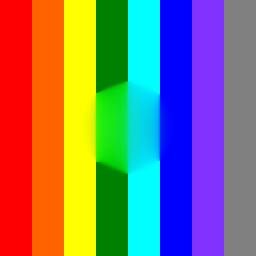
\includegraphics[width=0.8\linewidth]{images/result_ex1/fixpoint03.png}			
	\end{subfigure}
	\begin{subfigure}{0.4\linewidth}
		\centering
		
\includegraphics[width=0.8\linewidth]{images/result_ex1/fixpoint04.png}			
	\end{subfigure}
	\begin{subfigure}{0.4\linewidth}
		\centering
		
\includegraphics[width=0.8\linewidth]{images/result_ex1/fixpoint05.png}			
	\end{subfigure}
	\caption{ผลการซ่อมแซมจากวิธีการทำซ้ำแบบจุดตรึง}
\end{figure}
\begin{table}[H]
	\centering
	\begin{tabular}[ht]{|c|c|c|c|c|}
		\hline
		รูปภาพ &เวลาประมวล  (วินาที) & PSNR (dB) & SSIM \\
		\hline
		1 & 24.97 & 60.95 & 1.0000 \\ 
		2 & 53.06 & 37.69 & 1.0000 \\
		3 &  190.64 & 25.17 & 0.9997 \\
		4 & 50.63  & 28.81  & 0.9999 \\
		5 & 54.74  & 40.73  & 1.0000 \\
		\hline
		เฉลี่ย & 74.81  & 38.67  & 0.9999 \\
		\hline
	\end{tabular}
	\caption{ผลการซ่อมแซมของวิธีการทำซ้ำแบบจุดตรึง}
\end{table}	
\begin{figure}[H]
	\centering
	\begin{subfigure}{0.4\linewidth}
		\centering
		
\includegraphics[width=0.8\linewidth]{images/result_ex1/splitbergman01.png}
	\end{subfigure}
	\begin{subfigure}{0.4\linewidth}
		\centering
		
\includegraphics[width=0.8\linewidth]{images/result_ex1/splitbergman02.png}
	\end{subfigure}
	\begin{subfigure}{0.4\linewidth}
		\centering
		
\includegraphics[width=0.8\linewidth]{images/result_ex1/splitbergman03.png}			
	\end{subfigure}
	\begin{subfigure}{0.4\linewidth}
		\centering
		
\includegraphics[width=0.8\linewidth]{images/result_ex1/splitbergman04.png}			
	\end{subfigure}
	\begin{subfigure}{0.4\linewidth}
		\centering
		
\includegraphics[width=0.8\linewidth]{images/result_ex1/splitbergman05.png}			
	\end{subfigure}
	\caption{ผลการซ่อมแซมจากวิธีการสปริทเบรกแมน}
		\label{result:image-splitbregman}
\end{figure}
\begin{table}[H]
	\centering
	\begin{tabular}[ht]{|c|c|c|c|c|}
		\hline
		รูปภาพ &เวลาประมวล  (วินาที) & PSNR (dB) & SSIM \\
		\hline
		1 & 3.39 & 71.54 & 1.0000 \\ 
		2 & 10.74 & 37.08 & 1.0000 \\
		3 &  24.50 & 26.08 & 0.9997 \\
		4 & 15.80  & 29.61  & 0.9999 \\
		5 & 15.85  & 32.78  & 1.0000 \\
		\hline
		เฉลี่ย & 14.06  & 39.42  & 0.9999 \\
		\hline
	\end{tabular}
	\caption{ผลการซ่อมแซมของวิธีสปริทเบรกแมน}
	\label{result:table-splitbregman}
\end{table}
	\hspace{1cm} ประสิทธิภาพของวิธีการเชิงตัวเลขทั้ง 3 วิธี สามารถสรุปได้ดังนี้
	\begin{table}[H]
		\centering
		\begin{tabular}[ht]{|l|c|c|c|c|}
			\hline
			วิธีการ  & เวลาประมวล  (วินาที) & PSNR (dB) & SSIM \\
			\hline
			การเดินเวลา & 120.68 & 16.72 & 0.9960 \\
			การทำซ้ำจุดตรึง & 74.81 & 38.67 & 0.9999 \\
			การสปริทเบรกแมน & 14.06 & 39.42 & 0.9999  \\
			\hline
		\end{tabular}
		\caption{แสดงการซ่อมแซมเฉลี่ยของวิธีการเชิงตัวเลข}
	\end{table}	
	\hspace{1cm} 
	จากทั้ง 3 วิธีที่ได้ทดสอบ จะเห็นได้ว่าวิธีการสปริทเบรกแมนใช้เวลาน้อยกว่าวิธีอื่น และมีคุณภาพ ซึ่งพิจารณาจาก ค่า PSNR และค่า SSIM มากกว่าวิธีอื่น ผู้วิจัยจึงสนใจทำการปรับปรุงวิธีสปิทเบรกแมนให้มีประสิทธิภาพสูง
	
	\subsubsection{ขั้นตอนวิธีเชิงตัวเลขสำหรับต่อเติมภาพชนิดใหม่}
	\hspace{1cm} เพื่อให้วิธีการสปริทเบรกแมนประมวลผลภาพได้รวดเร็วขึ้น ผู้วิจัยได้พัฒนากระบวนการกำหนดคำตอบเริ่มต้น โดยวิธีการ มัลติรีโซลูชัน (multi-resolution method) หรือวิธีการพีระมิดรูปภาพ (pyramid method) \cite{ref:image-pyramid}
	เริ่มจากการย่อขนาดรูปลงครึ่งนึงโดยใช้วิธี Bilinear Interpolation จนกระทั่งถึงระดับความคมชัดที่ต้องการ จากนั้นทำการต่อเติมภาพขนาดเล็ก และนำผลลัพธ์ที่ได้จากภาพขนาดเล็กทำการขยายภาพขึ้นสองเท่าโดยใช้ Bilinear Interpolation เป็นคำตอบเริ่มต้นสำหรับการต่อเติมภาพในชั้นถัดไป
	 	\begin{figure}[H]
	 	\centering
	 	\begin{subfigure}{0.4\linewidth}
	 		\centering
	 		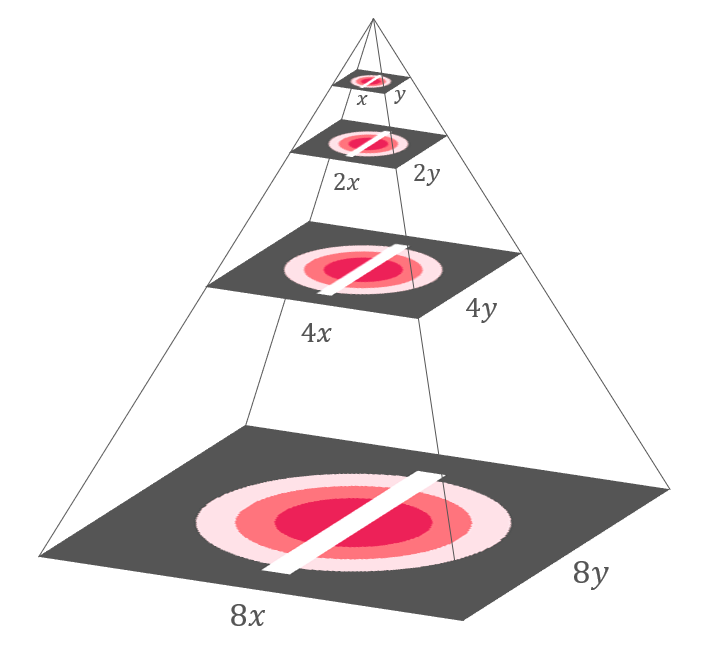
\includegraphics[width=0.8\linewidth]{images/image_inpaint_synthetic/image_pyramid.png}
	 	\end{subfigure}
 		 \caption{วิธีการพีระมิดรูปภาพ}
	 \end{figure}
 	\hspace{1cm} ขั้นตอนวิธีสำหรับการทำพีระมิดรูปภาพสำหรับการต่อเติมภาพแบบสปริทเบรกแมนเพื่อให้ประมวลผลได้เร็วขึ้นนั้นสามารถสรุปได้ดังนี้
	\begin{algorithm}[H]
		\label{algo:MultiSplitBregmanColorInpaint}
		\caption{Multi-resolution SB method}
		\SetAlgoNoLine
		\SetKwFunction{FMain}{$u \longleftarrow MRSBC $}
		\SetKwProg{Fn}{}{}{}
		\Fn{\FMain{$\boldsymbol{u}, \boldsymbol{z},\lambda, \theta, N_{gs}, N_0,N_1,N_2, \varepsilon,c,m$}}{
			\textbf{Initialize} $height = $ ความสูงของภาพ $\boldsymbol{u}$, $width = $ ความกว้างของภาพ $\boldsymbol{u}$ \\
			\If{c < m}{
				$\boldsymbol{x} = Bilinear(\boldsymbol{u},\lfloor width * 0.5 \rfloor,\lfloor height * 0.5 \rfloor)$\\
				$y = Bilinear(\lambda,\lfloor width * 0.5 \rfloor,\lfloor height * 0.5 \rfloor)$\\
				$r = MRSBC(\boldsymbol{x},\boldsymbol{z},y, \lambda, \theta,$ \\$ \hspace{1cm}  N_{gs}, N_0, N_1, N_2, \varepsilon,c+1,m)$\\
				$\boldsymbol{u} = Bilinear(r,width,height)$\\
			}
			\uIf{$c = 1$}{$N_{SB}=N_0$}
			\uElseIf{$c = m$}{$N_{SB} = N_2$}
			\Else{
				$N_{SB} = N_1$
			}
			$u = SBC(\boldsymbol{u}, \boldsymbol{z}, \lambda, \theta, N_{gs}, N_{SB}, \varepsilon) $  \\
		}
	\end{algorithm}
\begin{algorithm}[H]
		\caption{Bilinear Interpolation}
		\SetAlgoNoLine
		% https://stackoverflow.com/questions/26142288
		\SetKwFunction{FMain}{$J \longleftarrow Bilinear$}
		\SetKwProg{Fn}{}{}{}
		\Fn{\FMain{$I,x,y$}}{
			\textbf{Initialize}  $v =$ ความสูงของภาพ $I$, $w$ คือความกว้างของภาพ $I$,\\ $S_R = \frac{c}{a}, S_C = \frac{d}{b}, r = 1,2,...,v, c = 1,2,...,w,$\\$r' = 1,2,...x, c' = 1,2,...,y,  $ \\
			$r_f = \lfloor r' \cdot S_R \rfloor $\\
			$c_f = \lfloor c' \cdot S_C \rfloor $\\
			$\triangle r = r_f - r$ \\
			$\triangle c = c_f - c$ \\
			$J(r',c') = I(r,c)\cdot(1-\triangle r)\cdot (1-\triangle c) $\\$+ I(r+1,c) \cdot \triangle r \cdot (1 - \triangle c) $\\$+I(r,c+1)\cdot(1-\triangle r)\cdot\triangle c$\\$+ I(r+1,c+1)\cdot\triangle r \cdot \triangle c$ \\
		}
	\end{algorithm}
	\clearpage
	\hspace{1cm} ตารางที่ \ref{result:table-multiresolution1} แสดงผลการเปรียบเทียบประสิทธิภาพของขั้นตอนวิธีการที่ \ref{algo:MultiSplitBregmanColorInpaint} ภายใต้การเปลี่ยนแปลงจำนวนรอบของการทำซ้ำของวิธีการสปริทเบรกแมนบนภาพที่มีความคมชัด 256x256 พิกเซล ตัวอย่าง เช่น 10/3/3/10000 หมายถึงที่ระดับความคมชัดหยาบสุดซึ่งมีขนาดเป็น 32x32 พิกเซลจะทำซ้ำไม่เกิน 10 ครั้ง สำหรับที่ความคมชัดละเอียดขึ้นเป็น 64x64 พิกเซลจะทำซ้ำไม่เกิน 3 ครั้ง และสำหรับที่ระดับความคมชัดเป็น 128x128 พิกเซลจะทำซ้ำ 3 ครั้ง และที่ระดับความคมชัดเป็น 256x256 จะทำซ้ำไม่เกิน 10,000 ครั้งหรือจนค่าความคลาดเคลื่อนสัมพัทธ์ต่างกันไม่เกิน 0.0001 
	
	\begin{table}[H]
		\footnotesize
		\centering
		\begin{tabular}[ht]{|l|c|c|c|c|c|}
			\hline
			รูปแบบการทำซ้ำ  & รูปภาพ &เวลาประมวล  (วินาที) & PSNR (dB) & SSIM \\
			\hline
			ไม่ใช้พีระมิดรูปภาพ & 1 & 4.49  & 71.54 & 1.0000 \\ 
			& 2 & 13.16 & 37.08 & 1.0000 \\
			& 3 & 29.46 & 26.08 & 0.9997 \\
			& 4 & 20.50 & 29.61 & 0.9999 \\
			& 5 & 19.32 & 32.78 & 1.0000 \\
			\hline
			10/1/1/10000 & 1 & 2.44 & 69.59& 1.0000 \\
			& 2 & 11.31 &37.04 & 1.0000 \\
			& 3 & 23.48 & 27.34 & 0.9998 \\
			& 4 & 16.60 & 29.42 & 0.9999 \\
			& 5 & 13.75 & 33.53 & 1.0000 \\
			\hline
			10/3/3/10000  & 1 & 2.24 & 69.96 & 1.0000\\
			& 2 & 10.91 & 37.05 & 1.0000 \\
			& 3 & 21.99 & 27.66 & 0.9998 \\
			& 4 & 12.70 & 29.35 & 0.9999 \\
			& 5 & 11.49 & 33.69 & 1.0000\\
			\hline
			10/10/10/10000  & 1 & 1.83 & 71.58 & 1.0000 \\
			& 2 & 7.83 & 37.05 & 1.0000 \\
			& 3 & 16.75 & 28.62 & 0.9998 \\
			& 4 & 11.89 & 29.32 & 0.9999 \\
			& 5 & 8.00 & 34.26 & 1.0000 \\
			\hline
			100/1/1/10000  & 1 & 1.43 & 67.63 & 1.0000\\
			& 2 & 7.17 & 37.10 & 1.0000 \\
			& 3 & 20.86 & 27.70 & 0.9998 \\
			& 4 & 12.80 & 29.64 & 0.9999\\
			& 5 & 9.17 & 33.14 & 1.0000 \\
			\hline
			100/3/3/10000  & 1 & 1.68 & 71.18 & 1.0000 \\
			& 2 & 7.41 & 37.11 & 1.0000\\
			& 3 & 21.08 & 28.00 & 0.9998 \\
			& 4 & 13.28 & 29.38 & 0.9999 \\
			& 5 & 7.96 & 33.34 & 1.0000\\
			\hline
			100/10/10/10000  & 1 & 1.76 & 71.56 & 1.0000 \\
			& 2 & 7.32 & 37.04 & 1.0000\\
			& 3 & 16.62 & 28.65 & 0.9998 \\
			& 4 & 13.18 & 29.39 & 0.9999\\
			& 5 & 7.45 & 33.94 & 1.0000 \\
			\hline
		\end{tabular}
		\caption{ผลการซ่อมแซมภาพโดยวิธีการเชิงตัวเลขที่นำเสนอ}
		\label{result:table-multiresolution1}
\end{table}	
	\begin{table}[H]
		\centering
		\begin{tabular}[ht]{|l|c|c|c|c|}
			\hline
			รูปแบบการทำซ้ำ  & เวลาประมวล  (วินาที) & PSNR (dB) & SSIM \\
			\hline
			ไม่ใช้พีระมิดรูปภาพ & 17.38 & 39.42 & 0.9999 \\
			10/1/1/10000 & 13.52 & 39.38 & 0.9999 \\
			10/3/3/10000 & 11.86 & 39.54 & 0.9999 \\
			10/10/10/10000 & 9.26 & 40.17 & 0.9999\\
			100/1/1/10000 & 10.28 & 39.04 & 0.9999\\
			100/3/3/10000 & 10.28 & 39.80 & 0.9999\\
			100/10/10/10000 & 9.27 & 40.12 & 0.9999 \\
			\hline
		\end{tabular}
		\caption{ผลการซ่อมแซมภาพโดยวิธีการเชิงตัวเลขที่นำเสนอในรูปของค่าเฉลี่ยของผลที่ได้จากตารางที่ \ref{result:table-multiresolution1}}
		\label{result:table-multiresolution1-summary}
	\end{table}	
	
	\hspace{1cm}จากตารางที่ \ref{result:table-multiresolution1-summary} สังเกตว่า ยิ่งจำนวนการทำซ้ำในชั้นที่รูปภาพมีขนาดเล็กจำนวนมากครั้ง จะยิ่งทำให้เวลาประมวลผลที่ใช้ในการต่อเติมภาพใช้เวลาน้อยลง
	
	\hspace{1cm} นอกจากนี้แล้ว ผู้วิจัยยังได้สังเกตอีกว่า การทำซ้ำน จะลู่เข้าเร็วในช่วงแรก จากนั้นความเร็วในการลู่เข้าจะลดลง ซึ่งทำให้การทำซ้ำเพียงไม่กี่ครั้งในระดับความคมชัดเดิม  มีผลการซ่อมแซมภาพจนแสดงความคล้ายคลึงกับภาพต้นฉบับได้
	
	\begin{figure}[H]
		\centering
		\begin{subfigure}{0.4\linewidth}
			\centering
			
\includegraphics[width=0.7\linewidth]{images/just10enough/only5time.png}
			\caption{5 ครั้ง}
		\end{subfigure}
		\begin{subfigure}{0.4\linewidth}
			\centering
			
\includegraphics[width=0.7\linewidth]{images/just10enough/only10time.png}
			\caption{10 ครั้ง}
		\end{subfigure}
		\begin{subfigure}{0.4\linewidth}
			\centering
			
\includegraphics[width=0.7\linewidth]{images/just10enough/only50time.png}			
			\caption{50 ครั้ง}
		\end{subfigure}
		\begin{subfigure}{0.4\linewidth}
			\centering
			
\includegraphics[width=0.7\linewidth]{images/just10enough/only100time.png}			
			\caption{100 ครั้ง}
		\end{subfigure}
		\caption{พีระมิดที่ลำดับการทำซ้ำเป็น 10/10/10 และที่ระดับความคมชัดละเอียดสุดใช้จำนวนการทำซ้ำที่ต่างกัน}
	\end{figure}
	\clearpage
	 \hspace{1cm} ผู้วิจัยจึงกำหนดให้การทำซ้ำในระดับความละเอียดสุดเท่ากับ 10 ครั้ง และพบว่าได้ผลการซ่อมแซมดังตารางที่ \ref{result:table-multiresolution2}
		\begin{table}[H]
		\centering
		\small
		\begin{tabular}[ht]{|l|c|c|c|c|c|}
			\hline
			รูปแบบการทำซ้ำ  & รูปภาพ &เวลาประมวล  (วินาที) & PSNR (dB) & SSIM \\
			\hline
			ไม่ใช้พีระมิดรูปภาพ & 1 & 0.30  & 26.71  & 0.9998 \\ 
			& 2 & 0.39  & 18.39  & 0.9982 \\
			& 3 & 0.38 & 13.66  & 0.9944 \\
			& 4 & 0.40  & 12.86 & 0.9934 \\
			& 5 & 0.38 & 14.69 &  0.9956\\
			\hline
			10/1/1/10 & 1 & 0.29 & 40.10 & 1.0000\\
			& 2 & 0.41 & 31.28 & 0.9999 \\
			& 3 & 0.46 & 16.51 & 0.9970 \\
			& 4 & 0.47 & 26.56 & 0.9998\\
			& 5 & 0.39 & 28.25 & 0.9998 \\
			\hline
			10/3/3/10  & 1 & 0.28 & 42.53 & 1.0000\\
			& 2 & 0.36 & 32.91 & 1.0000 \\
			& 3 & 0.35 & 16.88 & 0.9972 \\
			& 4 & 0.34 & 27.06 &  0.9998 \\
			& 5 & 0.34 & 29.76 & 0.9999 \\
			\hline
			10/10/10/10  & 1 & 0.31 & 50.06 & 1.0000 \\
			& 2 & 0.41 & 34.01 & 1.0000\\
			& 3 & 0.38 & 18.19 & 0.9980\\
			& 4 & 0.39 & 27.50 & 0.9998\\
			& 5 & 0.40 & 33.05 &  1.0000\\
			\hline
			100/1/1/10  & 1 & 0.27 & 43.97 & 1.0000 \\
			& 2 & 0.37  & 31.28 & 0.9999\\
			& 3 & 0.36 & 24.98 & 0.9997\\
			& 4 & 0.36  &28.05 & 0.9998\\
			& 5 & 0.36 & 29.24 & 0.9999 \\
			\hline
			100/3/3/10  & 1 & 0.29 & 45.08& 1.0000 \\
			& 2 & 0.36 & 32.36 & 0.9999\\
			& 3 & 0.40 & 24.35 & 0.9996\\
			& 4 & 0.38 & 27.88 & 0.9998\\
			& 5 & 0.37 & 30.28 & 0.9999 \\
			\hline
			100/10/10/10  & 1 & 0.28 & 50.05 &  1.0000\\
			& 2 & 0.41 & 33.25 &  1.0000\\
			& 3 & 0.42 & 23.51 & 0.9995 \\
			& 4 & 0.42 & 27.78 & 0.9998 \\
			& 5 & 0.39 & 32.38 & 0.9999 \\
			\hline
		\end{tabular}
		\caption{ผลการซ่อมแซมภาพโดยวิธีการเชิงตัวเลขที่นำเสนอเมื่อใช้การทำซ้ำในระดับความคมชัดละเอียดสุด 10 ครั้ง}
		\label{result:table-multiresolution2}
	\end{table}	
	\begin{table}[H]
		\centering
		\begin{tabular}[ht]{|l|c|c|c|c|}
			\hline
			รูปแบบการทำซ้ำ  & เวลาประมวล  (วินาที) & PSNR (dB) & SSIM \\
			\hline
			ไม่ใช้พีระมิดรูปภาพ & 0.37 & 17.26 & 0.9963  \\
			10/1/1/10 & 0.40 & 28.54 & 0.9993 \\
			10/3/3/10 & 0.33 & 29.83  & 0.9994 \\
			10/10/10/10 & 0.38 & 32.56 & 0.9995 \\
			100/1/1/10 & 0.34 & 31.50 & 0.9999 \\
			100/3/3/10 & 0.36 & 31.99 & 0.9999 \\
			100/10/10/10 & 0.38 & 33.39 & 0.9998 \\
			\hline
		\end{tabular}
		\caption{ผลการซ่อมแซมภาพโดยวิธีการเชิงตัวเลขที่นำเสนอในรูปของค่าเฉลี่ยของผลที่ได้จากตารางที่ \ref{result:table-multiresolution2}}
		\label{result:table-multiresolution2-summary}
	\end{table}	

	\hspace{1cm}จากตารางจะเห็นว่า การทำซ้ำในชั้นที่รูปภาพมีขนาดเล็กมากจำนวนมาก ไม่ช่วยให้การประมวลผลได้เร็วขึ้น ผู้วิจัยจึงเลือกใช้การทำซ้ำแบบ 10/3/3/10 ในการต่อเติมภาพ
	
	\subsubsection{การทดสอบประสิทธิภาพในการซ่อมแซมภาพจิตรกรรมไทยโบราณ}
	\hspace{1cm}ภาพจิตรกรรมทีี่ใช้ทดสอบ มีทั้งสิ้น 5  ภาพ โดยแต่ละภาพเป็นภาพสีที่มีขนาด 256x256 พิกเซล ซึ่งทั้ง 5 ภาพได้แก่ ภาพที่ \ref{image:thaiart_case01_original} \footnote{ภาพถ่ายที่วัดแก้วไพฑูรย์; ภาพจาก  https://commons.wikimedia.org/wiki/File:จิตรกรรมฝาผนัง\_วัดแก้วไพฑูรย์\_(7).jpg สืบค้นเมื่อวันที่ 23 กันยายน 2561}   และภาพที่ \ref{image:thaiart_case02_original} \footnote{ภาพถ่ายที่วัดแก้วไพฑูรย์; ภาพจาก  https://commons.wikimedia.org/wiki/File:จิตรกรรมฝาผนัง\_วัดแก้วไพฑูรย์\_(2).jpg สืบค้นเมื่อวันที่ 23 กันยายน 2561} คือ จิตรกรรมฝาผนังวัดแก้วไพฑูรย์ ภาพที่ \ref{image:thaiart_case03_original} \footnote{ภาพถ่ายที่วัดพระยืนพุทธบาทยุคล; ภาพจาก https://commons.wikimedia.org/wiki/File:Wat\_Phra\_Yuen \_Phutthabat\_Yukhon\_01.jpg สืบค้นเมื่อวันที่ 23 กันยายน 2561}  คือ จิตรกรรมฝาผนังวัดพระยืนพุทธบาทยุคล ภาพที่ \ref{image:thaiart_case04_original} \footnote{ภาพถ่ายที่วัดคงคาราม; ภาพจาก  https://commons.wikimedia.org/wiki/File:จิตรกรรม\_อุโบสถวัดคงคาราม.JPG สืบค้นเมื่อวันที่ 23 กันยายน 2561} คือ จิตรกรรมฝาผนังวัดคงคาราม และภาพที่ \ref{image:thaiart_case05_original} \footnote{ภาพถ่ายที่วัดท่าถนน; ภาพจาก  https://commons.wikimedia.org/wiki/File:Wat\_Tha\_Thanon\_05.JPG สืบค้นเมื่อวันที่ 23 กันยายน 2561} คือ จิตรกรรมฝาผนังวัดท่าถนน
	โดยจะทำให้ข้อมูลข้องทั้ง 5 ภาพเกิดความเสียหาย โดยใช้รอยความเสียหายจากภาพพระเจ้าสร้างอดัม
	
	\begin{figure}[H]
		\centering
		\begin{subfigure}{0.4\linewidth}
			\centering
			
\includegraphics[width=0.8\linewidth]{images/thaiart/case01-original.png}
			\caption{วัดแก้วไพฑูรย์}
			\label{image:thaiart_case01_original}
		\end{subfigure}
		\begin{subfigure}{0.4\linewidth}
			\centering
			
\includegraphics[width=0.8\linewidth]{images/thaiart/case02-original.png}
			\caption{วัดแก้วไพฑูรย์}
			\label{image:thaiart_case02_original}
		\end{subfigure}
		\begin{subfigure}{0.4\linewidth}
			\centering
			
\includegraphics[width=0.8\linewidth]{images/thaiart/case03-original.png}
			\caption{วัดพระยืนพุทธบาทยุคล}
			\label{image:thaiart_case03_original}			
		\end{subfigure}		
		\begin{subfigure}{0.4\linewidth}
			\centering
			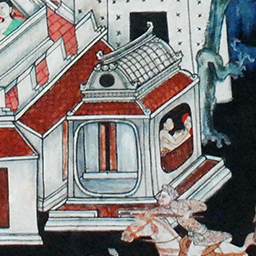
\includegraphics[width=0.8\linewidth]{images/thaiart/case04-original.png}
			\caption{วัดคงคาราม}
			\label{image:thaiart_case04_original}			
		\end{subfigure}
		\begin{subfigure}{0.4\linewidth}
			\centering
			
\includegraphics[width=0.8\linewidth]{images/thaiart/case05-original.png}
			\caption{วัดท่าถนน}
			\label{image:thaiart_case05_original}			
		\end{subfigure}
		\begin{subfigure}{0.4\linewidth}
			\centering
			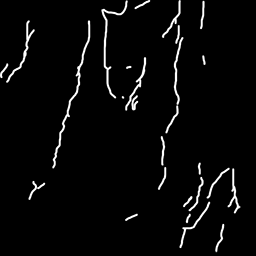
\includegraphics[width=0.8\linewidth]{images/thaiart/inpaint-domain.png}
			\caption{รอยความเสียหาย}
		\end{subfigure}
		\caption{ภาพต้นฉบับสำหรับใช้ในการทดสอบ}
	\end{figure}
	\begin{figure}[H]
	\centering
	\begin{subfigure}{0.4\linewidth}
		\centering
		
\includegraphics[width=0.8\linewidth]{images/thaiart/case01-toinpaint.png}
	\end{subfigure}
	\begin{subfigure}{0.4\linewidth}
		\centering
		
\includegraphics[width=0.8\linewidth]{images/thaiart/case02-toinpaint.png}
	\end{subfigure}
	\vspace{1cm}
	\begin{subfigure}{0.4\linewidth}
		\centering
		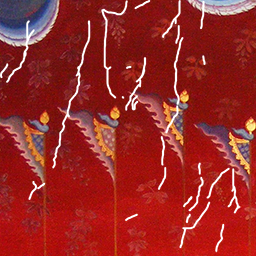
\includegraphics[width=0.8\linewidth]{images/thaiart/case03-toinpaint.png}			
	\end{subfigure}
	\begin{subfigure}{0.4\linewidth}
		\centering
		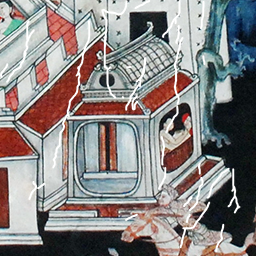
\includegraphics[width=0.8\linewidth]{images/thaiart/case04-toinpaint.png}			
	\end{subfigure}
	\begin{subfigure}{0.4\linewidth}
		\centering
		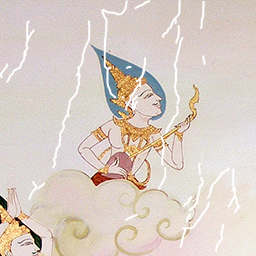
\includegraphics[width=0.8\linewidth]{images/thaiart/case05-toinpaint.png}			
	\end{subfigure}
	\caption{ภาพที่ทำให้เสียหาย}
\end{figure}
	 \hspace{1cm} จากนั้นทำการทดสอบการต่อเติมภาพทั้ง 5 โดยทดสอบวิธีสปริทเบรกแมน และวิธีทีที่พัฒนาขึ้นโดยใช้วิธีการสปริทเบรกแมนพร้อมทั้งการใช้พีระมิดรูปภาพที่มีการทำซ้ำแต่ละชั้นเป็น 10/3/3/10  ได้ผลลัพธ์ออกมาเป็นดังนี้
	\begin{figure}[H]
		\centering
		\begin{subfigure}{0.4\linewidth}
			\centering
			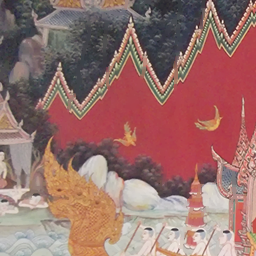
\includegraphics[width=0.8\linewidth]{images/result_ex4/splitbergman_case01.png}
		\end{subfigure}
		\begin{subfigure}{0.4\linewidth}
			\centering
			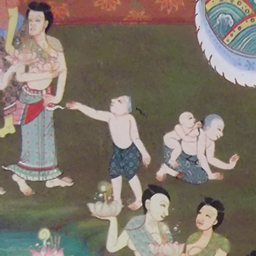
\includegraphics[width=0.8\linewidth]{images/result_ex4/splitbergman_case02.png}
		\end{subfigure}
		\begin{subfigure}{0.4\linewidth}
			\centering
			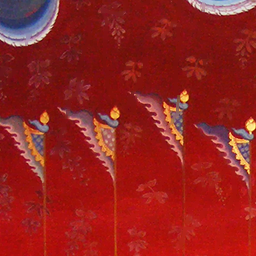
\includegraphics[width=0.8\linewidth]{images/result_ex4/splitbergman_case03.png}			
		\end{subfigure}
		\begin{subfigure}{0.4\linewidth}
			\centering
			\includegraphics[width=0.8\linewidth]{images/result_ex4/splitbergman_case04.png}			
		\end{subfigure}
		\begin{subfigure}{0.4\linewidth}
			\centering
			\includegraphics[width=0.8\linewidth]{images/result_ex4/splitbergman_case05.png}			
		\end{subfigure}
		\caption{ผลการซ่อมแซมโดยวิธีการสปริทเบรกแมน}
	\end{figure}
	\begin{table}[H]
		\centering
		\begin{tabular}[ht]{|c|c|c|c|c|}
			\hline
			รูปภาพ &เวลาประมวล  (วินาที) & PSNR (dB) & SSIM \\
			\hline
			1 & 2.95 & 33.92 & 1.0000 \\ 
			2 & 2.64 & 37.33 & 1.0000 \\
			3 &  3.49 & 37.21 & 1.0000 \\
			4 & 2.70  & 29.47  & 1.0000 \\
			5 & 15.85  & 32.78  & 1.0000 \\
			\hline
			เฉลี่ย & 2.72  & 34.89  & 1.0000 \\
			\hline
		\end{tabular}
		\caption{ผลการซ่อมแซมภาพศิลปะไทยจากวิธีการสปิทเบรกแมน}
		\label{result:table-thaiart-splitbregman}
	\end{table}
	\begin{figure}[H]
		\centering
		\begin{subfigure}{0.4\linewidth}
			\centering
			\includegraphics[width=0.8\linewidth]{images/result_ex4/multisplitbergman_case01.png}
		\end{subfigure}
		\begin{subfigure}{0.4\linewidth}
			\centering
			\includegraphics[width=0.8\linewidth]{images/result_ex4/multisplitbergman_case02.png}
		\end{subfigure}
		\begin{subfigure}{0.4\linewidth}
			\centering
			\includegraphics[width=0.8\linewidth]{images/result_ex4/multisplitbergman_case03.png}			
		\end{subfigure}
		\begin{subfigure}{0.4\linewidth}
			\centering
			\includegraphics[width=0.8\linewidth]{images/result_ex4/multisplitbergman_case04.png}			
		\end{subfigure}
		\begin{subfigure}{0.4\linewidth}
			\centering
			\includegraphics[width=0.8\linewidth]{images/result_ex4/multisplitbergman_case05.png}			
		\end{subfigure}
		\caption{ผลการซ่อมแซมภาพโดยวิธีการเชิงตัวเลขที่พัฒนาขึ้น}
	\end{figure}
		\begin{table}[H]
		\centering
		\begin{tabular}[ht]{|c|c|c|c|c|}
			\hline
			รูปภาพ &เวลาประมวล  (วินาที) & PSNR (dB) & SSIM \\
			\hline
			1 & 0.40 & 34.13 & 1.0000 \\ 
			2 & 0.40 & 38.18 & 1.0000 \\
			3 &  0.39 & 37.73 & 1.0000 \\
			4 & 0.38  & 29.38  & 1.0000 \\
			5 & 0.39  & 37.11  & 1.0000 \\
			\hline
			เฉลี่ย & 0.39  & 35.30  & 1.0000 \\
			\hline
		\end{tabular}
		\caption{ผลการซ่อมแซมภาพศิลปะไทยโดยวิธีการเชิงตัวเลขที่พัฒนาขึ้น}
		\label{result:table-thaiart-mutisplitbregman}
	\end{table}	 
	\hspace{1cm}ทั้งสองวิธี ได้ผลลัพธ์การซ่อมแซมภาพศิลปะไทยในรูปค่าเฉลี่ยออกมาดังนี้
	\begin{table}[H]
		\centering
		\begin{tabular}[ht]{|l|c|c|c|c|}
			\hline
			วิธีการ  & เวลาประมวล  (วินาที) & PSNR (dB) & SSIM \\
			\hline
			สปริทเบรกแมน & 2.72 & 34.89 & 1.0000 \\ 
			วิธีการที่พัฒนาขึ้น & 0.39 & 35.30 & 1.0000 \\
			\hline
		\end{tabular}
		\caption{แสดงผลการซ่อมแซมภาพศิลปะไทยในรูปค่าเฉลี่ยจากตารางที่ 		\ref{result:table-thaiart-splitbregman} และตารางที่ 		\ref{result:table-thaiart-mutisplitbregman} }
		\label{result:table-thaiart-summary}
	\end{table}	
	\hspace{1cm} จากตารางที่ \ref{result:table-thaiart-summary} จะเห็นได้ว่า วิธีที่พัฒนาขึ้นนั้นสามารถทำงานได้เร็วกว่าวิธีสปริทเบรกแมนเดิม และยังมีคุณภาพที่ดีขึ้นด้วย
	
	
	
	\subsection{การลบบทบรรยายบนอนิเมะ}
	\hspace{1cm} สำหรับการลบบทบรรยายอนิเมะ จะใช้วิดีโอ Anime Festival Asia Special Video - feat. Inori Aizawa ซึ่งผลิตโดย Collateral Damage Studios โดยจะตัดวิดีโอ 1 นาทีแรกสำหรับการทดลอง โดยวิดีโอดังกล่าวขนาด 1280 x 720 พิกเซล แต่เนื่องจากโดยปกติแล้ว อนิเมะมักมีบรรทัดเพียง 1 ถึง 2 บรรทัด จึงทำการแบ่งวิดีโอออกอีกเป็น 5 ส่วนได้ขนาดเป็น 1280 x 144 พิกเซลก่อนนำไปทดสอบในลำดับถัดไป
	\hspace{1cm} และสำหรับบทบรรยายที่จะใช้ทดสอบนั้น เนื่องจากวิดีโอ Anime Festival Asia Special Video - feat. Inori Aizawa ไม่มีคำพูดใดๆ จึงใช้บทความ lorem ipsum เป็นบทบรรยาย โดยจะทำการแสดงบทบรรยาย 1 บรรทัด ความยาว 3 วินาที ทุก 2 วินาที นั่นคือในวิดีโอดังกล่าวจะมีบทบรรยายทั้งสิ้น 20 บรรทัด	
	
	\begin{figure}[H]
		\centering
		\begin{subfigure}{0.8\linewidth}
			\centering
			\includegraphics[width=0.8\linewidth]{images/inori-subbed-preview.png}
		\end{subfigure}
		\caption{การแบ่งไฟล์วิดีโอเป็น 5 ส่วนสำหรับใช้เป็น 5 ชุดทดสอบ}
	\end{figure}
	
	\hspace{1cm}เนื่องจากไฟล์วิดีโอนั้นประกอบด้วยชุดของภาพหลายภาพ กล่าวคือ $V = \{\boldsymbol{u}_i| i = 1,2,3 ... N_f\}$ ทำให้ขั้นตอนวิธีการลบคำบรรยายออกจากวิดีโอ จะต้องทำการต่อเติมบริเวณที่เป็นบทบรรยายทีละภาพ ดังที่แสดงในขั้นตอนวิธีต่อไปนี้ \\
	
	\begin{algorithm}[H]
		\caption{Removing subtitle from video}	
		\SetAlgoNoLine
		\SetKwFunction{FMain}{$V \longleftarrow RemoveS$}
		\SetKwProg{Fn}{}{}{}
		\Fn{\FMain{$V$}}{
			\For{$ i = 1,2,... N_f$}{
				$\bullet$ หาโดเมนต่อเติม $D$ จาก $\boldsymbol{u}_i$\\
				$\bullet$ ต่อเติมภาพ $\boldsymbol{u}_i$ โดยใช้โดเมนต่อเติม $D$\\
			}
		}
	\end{algorithm}
	\vspace{1cm}
	\hspace{1cm} โดยขั้นตอนการต่อเติมภาพ $\boldsymbol{u}_i$ ด้วยโดเมนต่อเติม $D$ นั้นจะสามารถใช้วิธีการเดียวกับการซ่อมแซมภาพศิลปะไทยได้ ส่วนการหาบทบรรยายอนิเมะ จะกล่าวถึงในหัวข้อย่อย
	
	
	\subsubsection{การหาบทบรรยายบนอนิเมะ}	
	\hspace{1cm}ก่อนจะลบบทบรรยายนั้น จำเป็นต้องหาบทบรรยายในภาพให้ได้เสียก่อน โดยบทบรรยายของอนิเมะนั้น มักจะใช้ขอบของตัวอักษรเป็นสีดำ อีกทั้งบทบรรยายนั้นจะลอยห่างออกมาจากขอบของวิดีโอ และขนาดของคำบรรยายนั้นจะมีขนาดอยู่ประมาณหนึ่งไม่ใหญ่หรือไม่เล็กเกินไป ด้วยสมบัตินี้เองทำให้จึงสามารถหาบริเวณบนเฟรมที่เป็นบทบรรยายได้โดยจะมีวิธีหาพื้นที่ซึ่งเป็นบทบรรยายดังนี้
	
	\vspace{1cm}
	
	\begin{algorithm}[H]
		\caption{Finding subtitle}
		\SetKwFunction{FMain}{$D \longleftarrow findsub$}
		\SetAlgoNoLine
		\SetKwProg{Fn}{}{}{}
		\Fn{\FMain{$\boldsymbol{u}$}}{
			$\bullet$ ทำการเปลี่ยนสีดำในภาพ $\boldsymbol{u}$ ให้เป็นสีขาวแล้วเปลี่ยนอื่นๆ ให้เป็นสีดำเพื่อหาขอบของคำบรรยาย\\
			$\bullet$ เปลี่ยนบริเวณสีขาวในภาพให้เป็นสีดำ และเปลี่ยนบริเวณสีดำให้เป็นสีขาว\\
			$\bullet$ ทำการลบบริเวณสีขาวซึ่งติดกับขอบของภาพออกไป เนื่องจากบทบรรยายจะลอยอยู่ ไม่ติดกับขอบเสมอ\\
			$\bullet$  ลบบริเวณที่ใหญ่เกินกว่าจะเป็นบทบรรยาย \\
			$\bullet$  ลบบริเวณที่เล็กเกินกว่าจะเป็นบทบรรยาย \\
			$\bullet$ ทำการขยายพื้นที่ๆ เป็นสีขาวขึ้นด้วยความกว้างของขอบบทบรรยาย \\
			$\bullet$ สีขาวที่เหลืออยู่ในภาพจะเป็นบทบรรยาย
		}	
	\end{algorithm}
	\clearpage
	\hspace{1cm} วิธีการหาบทบรรยายที่กล่าวไปข้างต้น จะทำการทดสอบกับบทความ lorem ipsum\footnote{Cicero, De finibus bonorum et malorum; เข้าถึงได้ทาง https://en.wikipedia.org/wiki/Lorem\_ipsum สืบค้นเมื่อวันที่ 23 ตุลาคม 2561} ที่ถูกแปลเป็นภาษาไทย ภาษาอังกฤษ และภาษาญี่ปุ่น โดยมีความสามารถในการหาโดเมนต่อเติมใบบทบรรยายภาษาต่างๆ ดังนี้
	\begin{table}[H]
		\centering
		\footnotesize
		\begin{tabular}[ht]{|l|c|c|c|c|c|}
			\hline
			ภาษา  & วีดีโอ & จำนวนพิกเซลในโดเมน & จำนวนพิกเซลที่ตรวจพบ & จำนวนพิกเซลที่ผิดพลาด & ร้อยละการผิดพลาด \\
			\hline
			ไทย & 1 & 23,190,522  & 24,044,004 & 2,108,772 &9.09\\
				 & 2 & 23,232,287 & 24,026,820 & 2,204,025 & 9.49\\
				& 3 & 23,189,082 & 24,300,589 & 2,081,340 & 8.98\\
				& 4 & 23,277,706 & 23,796,276  & 2,126,004 & 9.13\\
				& 5 & 23,221,502 & 24,247,935 & 2,185,864 & 9.41\\
			\hline
			อังกฤษ & 1 & 27,281,185 & 28,631,063 & 3,477,960  & 12.75\\
			& 2 & 27,269,671 & 28,513,248 & 3,514,859 & 12.89\\
			& 3 & 27,325,148 & 28,611,300 & 3,815,082 & 13.96\\
			& 4 & 27,191,136 & 28,527,105 & 3,854,121 & 14.17\\
			& 5 & 27,326,584 & 28,709,405 & 3,909,582 & 14.31\\
			\hline
			ญี่ปุ่น & 1 & 28,509,908 & 30,058,101 &  3,953,067 & 13.87\\
			& 2 & 28,534,363  & 30,023,923 & 3,565,609 & 12.50\\
			& 3 & 28,537,968 & 30,015,047 & 3,553,128 & 12.45\\
			& 4 & 28,579,778 & 30,065,985 & 3,961,319 & 13.86\\
			& 5 & 28,558,848 & 30,354,275 & 3,671,730 & 12.86\\
			\hline
		\end{tabular}
		\caption{ความคลาดเคลื่อนของการหาโดเมนต่อเติม ในบทบรรยายภาษาต่างๆ}
	\end{table}
	\begin{table}[H]
		\centering
			\footnotesize
		\begin{tabular}[ht]{|l|c|c|c|c|}
			\hline
			ภาษา  & จำนวนพิกเซลในโดเมน & จำนวนพิกเซลที่ตรวจพบ & จำนวนพิกเซลที่ผิดพลาด & ร้อยละการผิดพลาด \\
			\hline
			ไทย & 23,222,220 & 24,083,125 & 2,141,201 & 9.22 \\
			อังกฤษ & 27,278,745 & 28,598,424 & 3,714,321 & 13.62 \\
			ญี่ปุ่น & 28,544,173 & 30,103,466 & 3,740,971 & 13.11 \\
			\hline
		\end{tabular}
		\caption{ความคลาดเคลื่อนเฉลี่ยของการหาโดเมนต่อเติม ในบทบรรยายภาษาต่างๆ}
	\end{table}	
	
	\hspace{1cm} จากการทดลองทั้ง  3 ภาษาพบว่าวิธีการหาคำบรรยายนี้ มีร้อยละการผิดพลาดเฉลี่ยอยู่ที่ 11.98 ซึ่งการทดลองจากนี้ไปจะใช้วิธีการหาคำบรรยายนี้ในการหาโดเมนต่อเติมแบบอัตโนมัติ
	\clearpage
	\subsubsection{การลบคำบรรยายจากบทอนิเมะ}
	\hspace{1cm} สำหรับอนิเมะนั้น แต่ละเฟรมจะเป็นรูปภาพ เราจึงสามารถประยุกต์ใช้วิธีการซ่อมแซมภาพจิตรกรรมไทย มาใช้ในการลบคำบรรยายได้ แต่ผู้วิจัยก็ได้สังเกตว่า สำหรับอนิเมะที่เป็นวิดีโอแล้ว ในขณะที่ประมวลผลวิดีโอ เราสามารถใช้ผลการต่อเติมภาพจากภาพที่แล้ว มาใช้เป็นคำตอบเริ่มต้นจึงได้ว่าขึ้นตอนการลบบทบรรยายออกจากวิดีโอมีดังนี้\\
	
			\vspace{0.5cm}
	
	\begin{algorithm}[H]
		\SetAlgoNoLine
		\caption{Removeing subtitle from video (Method 1)}
		\SetKwFunction{FMain}{$V \longleftarrow removeS1$}
		\SetKwProg{Fn}{}{}{}
		\Fn{\FMain{$V$}}{
			\textbf{initialize} $i =1$\\
			\While{$i < N_f - 1$}{
				$\boldsymbol{u}_i$ คือเฟรมที่ $i$ ใน $V$ \\
				$\boldsymbol{u}_{i+1}$ คือเฟรมที่ $i+1$ ใน $V$ \\
				$D$ คือโดเมนต่อเติมใน $\boldsymbol{u}_{i+1}$ \\
				$\boldsymbol{u}_{i+1} = removeS2(\boldsymbol{u}_{i},D,\boldsymbol{u}_{i+1})$
			}
		}	
	\end{algorithm}
	\vspace{0.5cm}
	\hspace{1cm}  $removeS2(\boldsymbol{u}_{i},D,u_{i+1})$  คือขั้นตอนวิธีที่ \ref{algo:borrowframe} ซึ่งในทำนองเดียวกันเราสามารถเปลี่ยน $removeS2(u_{i},D,\boldsymbol{u}_{i+1})$ เป็น $removeS3(\boldsymbol{u}_{i},D,u_{i+1})$ เพื่อใช้กับขั้นตอนวิธี \ref{algo:skipframe} และเปลี่ยนเป็น  $removeS4(\boldsymbol{u}_{i},D,\boldsymbol{u}_{i+1})$ เพื่อใช้กับขั้นตอนวิธี \ref{algo:skipnborrowframe} ได้ \\
	
	\vspace{0.5cm}
	
	\hspace{1cm} ขั้นตอนวิธี การยืมเฟรม จะเป็นการนำผลลัพธ์จากเฟรมก่อนหน้ามาเป็นคำตอบในการเริ่มต้นในการประมวลผลเพื่อให้ผลลัพธ์ลู่เข้าได้เร็วขึ้น \\
	
		\vspace{0.5cm}
	
	\begin{algorithm}[H]
		\SetAlgoNoLine
		\label{algo:borrowframe}
		\caption{Removing subtitle from video (Method 2)}  
		\SetKwFunction{FMain}{$\boldsymbol{v} \longleftarrow removeS2$}
		\SetKwProg{Fn}{}{}{}
		\Fn{\FMain{$\boldsymbol{u} , D, \boldsymbol{v} $}}{
			$s =$ ค่า SSIM ระหว่าง  $\boldsymbol{u}$ และ $\boldsymbol{v}$  บริเวณนอกโดเมนต่อเติม\\
			\If{s > 0.9}{
				คัดลอกบริเวณในโดเมนต่อเติมจาก $\boldsymbol{u} $ ไปยัง $\boldsymbol{z}$
			}
			$\boldsymbol{v} = MRSBC(\boldsymbol{u} ,\boldsymbol{z} ,\lambda, \theta, N_{gs}, N_0, N_1, N_2, \varepsilon,1,m)$
		}	
	\end{algorithm}
	\clearpage
	\hspace{1cm}ขั้นตอนวิธี การข้ามเฟรม สำหรับเฟรมใดที่ผลลัพธ์ใกล้เคียงกันมาก จะทำการข้ามการต่อเติมภาพในเฟรมนั้นไปโดยใช้คำตอบจากเฟรมก่อนหน้าแทนเพื่อลดเวลาการประมวลผล \\ 
	\vspace{0.5cm}
	\begin{algorithm}[H]
		\SetAlgoNoLine
		\label{algo:skipframe}
		\caption{Removeing subtitle from video (Method 3)}  
		\SetKwFunction{FMain}{$\boldsymbol{v}, \longleftarrow removeS3$}
		\SetKwProg{Fn}{}{}{}
		\Fn{\FMain{$\boldsymbol{u}, D, \boldsymbol{v}$}}{
			$s =$ ค่า SSIM ระหว่าง  $\boldsymbol{u}$ และ $\boldsymbol{v}$  บริเวณนอกโดเมนต่อเติม\\
			\uIf{s > 0.95}{
				คัดลอกบริเวณในโดเมนต่อเติมจาก $\boldsymbol{u}$ ไปยัง $\boldsymbol{v}$
			}
			\Else{
				$\boldsymbol{v} = MRSBC(\boldsymbol{u} ,\boldsymbol{z} ,\lambda, \theta, N_{gs}, N_0, N_1, N_2, \varepsilon,1,m)$
			}
		}	
	\end{algorithm}
	\vspace{0.5cm}
	\hspace{1cm}ขั้นตอนวิธี การข้ามและยืมเฟรม คือขั้นตอนวิธี \ref{algo:borrowframe} และขั้นตอนวิธี \ref{algo:skipframe} ที่นำมาประยุกต์ใช้งานร่วมกัน\\
	\vspace{0.5cm}
	\begin{algorithm}[H]
		\label{algo:skipnborrowframe}
		\caption{Removing subtitle from video (Method 4)}  
		\SetAlgoNoLine
		\SetKwFunction{FMain}{$\boldsymbol{v} \longleftarrow removeS4$}
		\SetKwProg{Fn}{}{}{}
		\Fn{\FMain{$\boldsymbol{u} , D, \boldsymbol{v} $}}{
			$s =$ ค่า SSIM ระหว่าง  $u$ และ $v$  บริเวณนอกโดเมนต่อเติม\\
			\uIf{s > 0.95}{
				คัดลอกบริเวณในโดเมนต่อเติมจาก $\boldsymbol{u} $ ไปยัง $\boldsymbol{v}$
			}
			\uElseIf{s > 0.9}{
				คัดลอกบริเวณในโดเมนต่อเติมจาก $\boldsymbol{u} $ ไปยัง $\boldsymbol{z}$\\
				$\boldsymbol{v} = MRSBC(\boldsymbol{u} ,\boldsymbol{z} ,\lambda, \theta, N_{gs}, N_0, N_1, N_2, \varepsilon,1,m)$
			}\Else{
				$\boldsymbol{v} = MRSBC(\boldsymbol{u} ,\boldsymbol{z} ,\lambda, \theta, N_{gs}, N_0, N_1, N_2, \varepsilon,1,m)$
			}
		}	
	\end{algorithm}
	\vspace{0.5cm}
	\hspace{1cm}ซึ่งผลลัพธ์เปรียบเทียบระหว่างแบบใช้วิธี ยืมเฟรม ใช้วิธีข้ามเฟรม และวิธีข้ามและยืมเฟรม ได้ผลดังตาราง
		\begin{table}[H]
		\small
		\centering
		\begin{tabular}[ht]{|l|c|c|c|c|c|}
			\hline
			วิธีการ  & วิดีโอ &เวลาประมวล  (วินาที) & PSNR (dB) & SSIM \\
			\hline
			สปริทเบรกแมน & 1 & 130.03  & 32.19 & 0.9528  \\ 
			และพีระมิดรูปภาพ& 2 & 135.17 & 29.98 & 0.9488 \\
			(ขั้นตอนวิธี \ref{algo:MultiSplitBregmanColorInpaint})& 3 & 142.11 & 30.54 & 0.9485 \\
			& 4 & 151.42 & 30.79 & 0.9494 \\
			& 5 & 147.70 & 33.48 & 0.9556 \\
			\hline
			ยืมเฟรม & 1 & 127.77  & 33.13& 0.9701 \\ 
			(ขั้นตอนวิธี \ref{algo:borrowframe})& 2 & 137.54 & 30.21 & 0.9590 \\
			& 3 & 124.71 & 31.43 & 0.9620 \\
			& 4 & 136.71 & 31.66 & 0.9614 \\
			& 5 & 137.16 & 34.56 &  0.9748 \\
			\hline
			ข้ามเฟรม & 1 &  104.55 & 27.10 &  0.9429\\ 
			(ขั้นตอนวิธี \ref{algo:skipframe})& 2 & 78.07 & 27.17 & 0.9351 \\
			& 3 & 73.35 & 29.21 & 0.9393\\
			& 4 & 116.20 & 29.91 & 0.9423 \\
			& 5 & 74.28 & 31.95 &  0.9442\\
			\hline
			ข้ามและยืมเฟรม & 1 & 68.11 & 27.24 & 0.9424 \\ 
			(ขั้นตอนวิธี \ref{algo:skipnborrowframe})& 2 & 73.91 & 27.22 & 0.9386 \\
			& 3 & 77.34 & 29.36 & 0.9437 \\
			& 4 & 81.98 & 30.35 & 0.9483  \\
			& 5 & 77.45  & 32.46 & 0.9540 \\
			\hline
		\end{tabular}
		\label{result:table-removesub1}
		\caption{ผลการลบบทบรรยายออกจากอนิเมะด้วยวิธีการเชิงตัวเลขขั้นตอนวิธี \ref{algo:MultiSplitBregmanColorInpaint}, \ref{algo:borrowframe}, \ref{algo:skipframe} และ \ref{algo:skipnborrowframe}}
	\end{table}	
	\begin{table}[H]
		\centering
		\begin{tabular}[ht]{|l|c|c|c|c|}
			\hline
			วิธีการ  & เวลาประมวล  (วินาที) & PSNR (dB) & SSIM \\
			\hline
			สปริทเบรกแมนและพีระมิดรูปภาพ & 141.29 & 31.39  &  0.9510\\
			ยืมเฟรม & 132.78 & 32.20 & 0.9655\\
			ข้ามเฟรม & 89.29 & 29.07 & 0.9408 \\
			ยืมเฟรมและข้ามเฟรม & 75.76 & 29.33 & 0.9454 \\
			\hline
		\end{tabular}
		\caption{ผลการซ่อมแซมภาพโดยวิธีการเชิงตัวเลขที่นำเสนอในรูปของค่าเฉลี่ยของผลที่ได้จากตารางที่ \ref{result:table-removesub1}}
	\end{table}	
	
	\hspace{1cm}  จากนั้นทำการทดสอบการต่อเติมวิดีโอทั้ง 5 โดยวิธีที่คิดค้นขึ้นใช้วิธีการสปริทเบรกแมนพร้อมทั้งการใช้พีระมิดรูปภาพที่มีการทำซ้ำแต่ละชั้นเป็น 10/3/3/10  พร้อมทั้งใช้การข้ามเฟรมและยืมเฟรม ได้ผลลัพธ์ออกเป็นดังตารางนี้
	 
\begin{table}[H]
	\centering
	\begin{tabular}[ht]{|l|c|c|c|c|}
		\hline
		วิธีการ  & เวลาประมวล  (วินาที) & PSNR (dB) & SSIM \\
		\hline
		สปริทเบรกแมน & * & * & * \\
		วิธีการที่พัฒนาขึ้น & 75.76 & 29.33 & 0.9454 \\
		\hline
	\end{tabular}
	\caption{ผลการลบบทบรรยายออกจากอนิเมะโดยวิธีการสปริทเบรกแมนและวิธีการที่พัฒนาขึ้น}
\end{table}	

\hspace{1cm} สำหรับวิธีสปริทเบรกแมน เนื่องจากใช้เวลา 1 ชั่วโมงแล้วยังประมวลผลวิดีโอชุดทดสอบแรกไม่เสร็จ ทางผู้พัฒนาจึงตัดสินใจยุติการทดลอง เนื่องจากอาจต้องใช้เวลาการประมวลผลเป็นเวลาหลายชั่วโมงสำหรับวิดีโอความยาว 1 นาที ส่วนวิธีที่คิดค้นขึ้น พบว่าสำหรับวิดีโอที่มีความยาว 1 นาที สามารถทำงานได้เสร็จอย่างรวดเร็ว โดยใช้เวลาเพียง 75 วินาที

\section{แผนการดำเนินงานวิจัย}
\hspace{1cm} แผนการดำเนินงานตลอดทั้งโครงการสามารถสรุปได้โดยย่อจากตารางต่อไปนี้
\begin{center}
	\scalebox{0.8}{\begin{tabular}[ht]{|l|c|c|c|c|c|c|c|c|c|c|c|c|}
			\hline
			&\multicolumn{12}{c|}{เดือนที่}\\
			\cline{2-13}
			แผนการดำเนินงาน&1&2&3&4&5&6&7&8&9&10&11&12\\
			\hline
			ศึกษาตัวแบบและขั้นตอนวิธีการต่อเติมภาพที่ใช้การแปรผันรวมในเชิงลึก&x&x& & & & & & & & & &\\
			พัฒนาขั้นตอนวิธีสำหรับการต่อเติมภาพที่ใช้การแปรผันรวมชนิดใหม่& & &x&x&x&x& & & & & &\\
			ทดสอบขั้นตอนวิธีการต่อเติมภาพที่พัฒนาขึ้นโดยโปรแกรม- & & & &x &x&x& & & & & &\\
			คอมพิวเตอร์บนภาพสังเคราะห์และภาพจริง & & & & & & & & & & & &\\
			อภิปรายผลที่ได้จากการทดลองเชิงตัวเลข & & & & & &x&x&x& & & &\\
			สรุปผลการดำเนินงานวิจัยและจัดทำรูปเล่มฉบับสมบูรณ์& & & & & & & & &x&x&x&x\\
			\hline
	\end{tabular}}
\end{center}


\section{บรรณานุกรม}

\renewcommand{\section}[2]{} % addition mod: remove reference text
\begin{thebibliography}{}
	
	\bibitem{ref:rof-inpaint-chan-shen} 
	T.F. Chan and J. Shen , “Mathematical models of local non-texture inpaintings”, SIAM Journal on Applied Mathematics, vol. 62, no. 3, pp. 1019–1043, 2001. 
	%\url{http://www.jstor.org/stable/3061798}
	
	\bibitem{ref:ROF-template} 
	L. I. Rudin, S. Osher, E. Fatemi, “Nonlinear total variation based noise removal algorithms", Physica D: Nonlinear Phenomena, vol 60, issues 1–4, pp. 259-268, 1992. 
	%\url{https://doi.org/10.1016/0167-2789(92)90242-F}
	
	\bibitem{ref:FixpointSolver}
	C.R. Vogel and M.E. Oman,“Iterative methods for total variation denoising", SIAM Journal on Scientific Computing. vol. 17, pp. 227-238, 1996.
	
	\bibitem{ref:splitbergman-inpaint}
	T. Goldstein and S. Osher,“The Split Bregman Method for L1-Regularized Problems", SIAM Journal on Imaging Sciences. vol. 2, issue 2, pp. 323-343, 2009.
	
	\bibitem{ref:image-pyramid}
	E.H. Andelson and C.H. Anderson and J.R. Bergen and P.J. Burt and J.M. Ogden. "Pyramid methods in image processing". 1984
	% วิกิ บอกว่าให้ ref ของคุณ Andelson
	% doi 10.1.1.56.8646
	%\url{https://en.wikipedia.org/wiki/Pyramid_(image_processing)#cite_ref-1}
	%\url{https://en.wikipedia.org/wiki/Multiresolution_analysis}
	
	\bibitem{ref:PSNR}
	David Salomon. Data Compression: The Complete Reference (4 ed.). Springer. pp. 281. 2007.
	%ISBN 978-1846286025.  \url{https://books.google.co.th/books?id=ujnQogzx_2EC&lpg=PA281&ots=FolwqB8qsN&dq=PSNR+infinite&pg=PA281&redir_esc=y#v=onepage&q=PSNR%20infinite&f=false}
	
	\bibitem{ref:SSIM}
	Zhou Wang, Alan Conrad Bovik, Hamid Rahim Sheikh and Eero P. Simoncelli, "Image quality assessment: from error visibility to structural similarity," in IEEE Transactions on Image Processing, vol. 13, no. 4, pp. 600-612, 2004.
	%\url{https://doi.org/10.1109/TIP.2003.819861}
	
\end{thebibliography}
\end{document}
	
	
	
	